\documentclass[a4paper,11pt]{jsreport}

\usepackage{comment}
\usepackage{float}
\usepackage{color}
\usepackage{multicol}
\usepackage[dvipdfmx]{graphicx}
\usepackage{wrapfig}
\usepackage{graphicx} 
\usepackage{tikz}
\usepackage{bm}
\usepackage{url}
\usepackage{underscore}
\usepackage{colortbl}
\usepackage{tabularx}
\usepackage{fancyhdr}
\usepackage{ulem}
\usepackage{cite}
\usepackage{amsmath,amssymb,amsfonts}
\usepackage{algorithmic}
\usepackage{textcomp}
\usepackage{xcolor}
\usepackage{braket}
\usepackage[ipaex]{pxchfon}
\usepackage[dvipdfmx]{hyperref} % ハイパーリンク
\usepackage{pxjahyper}
\usepackage[version=4]{mhchem} % 化学式をかくため
\usepackage[hang,small,bf]{caption}
\usepackage[subrefformat=parens]{subcaption}
\hypersetup{
setpagesize=false,
 bookmarksnumbered=true,%
 bookmarksopen=true,%
 colorlinks=true,%
 linkcolor=black,
 citecolor=black,
} % 目次の赤線を表示させないようにする
\captionsetup{compatibility=false}
\usetikzlibrary{positioning, intersections, calc, arrows.meta,math} %tikzのlibrary

\begin{document}

\thispagestyle{empty}
\begin{center}

  \vspace{20mm}
  {\Large\noindent 2024年度 修士論文}\\
  \vspace{40mm}
  {\Huge\noindent\textbf{機械学習を用いた}}\\
  \medskip
  {\Huge\noindent\textbf{イジング模型の相転移検出}}\\
  \vspace{\baselineskip}
  \vspace{40mm}

  {\Large\noindent
    2024年2月2日\\
    \vspace{\baselineskip}
    指導教員 \ 藤原高徳    \\
    \vspace{\baselineskip}
    茨城大学大学院\\
    理工学研究科 \ 量子線科学専攻 \\
    \vspace{\baselineskip}
    学籍番号 \ 22NM021S \\
    氏名 \ 須賀 勇貴\\
  }
  \vspace{40mm}

\end{center}

\thispagestyle{empty}
\clearpage

%=====================================================================================
\renewcommand{\abstractname}{要旨}

\begin{abstract}
  研究の要旨を書く.
\end{abstract}

\thispagestyle{empty}
\clearpage

%=====================================================================================

% 目次の表示
\tableofcontents

%=====================================================================================
\pagestyle{fancy}
\lhead{\rightmark}
\renewcommand{\chaptermark}[1]{\markboth{第\ \normalfont\thechapter\ 章~~#1}{}}
%=====================================================================================
\chapter{はじめに} %章
\section{研究背景}
\section{研究目的}


\chapter{イジング模型の相転移}
\section{相転移,臨界現象とは}
\subsection{物質の三態と相転移}
私たちにとって身近な物質である水(\ce{H2O})は,固体(氷),液体(水),気体(水蒸気)の3つの状態をとる.これら状態は温度の違いによって明確な規則性があり,1気圧の環境であれば,氷を徐々に温めていくと,ちょうど0℃で氷から水へ相転移がおき,さらにその水を温めておけば,ちょうど100℃で水から水蒸気への相転移が起きる.特に1気圧の環境では,1気圧の環境では,水と氷が共存しうるのはちょうど0℃に限られ,水と水蒸気が共存するのはちょうど100℃に限られる.これが摂氏という温度目盛りの基準になっていることは言うまでもない.\par
液体の水の温度が0℃から100℃に変化する間,密度や粘性などの水の物性は少しずつ変化する.しかし,これはあくまでも定量的な変化であり,水から氷,水から水蒸気への変化のような定性的な(あるいは質的な)変化とは違う.氷と水蒸気のそれぞれの範囲内での変化も,やはり質的な変化を伴わない,定量的な変化である.このように,定性的な変化を伴わずに移り変われるような一連の状態をひとまとめにして,相(Phase)と呼ぶ.氷,水,水蒸気はそれぞれ固相,液相,気相という三つの相に対応する.温度などのパラメータを変化させたときに,物質が異なった相の間を移り変わる現象を相転移(phase transition)である.\par
なぜ同じ\ce{H2O}という物質が,温度を変えただけで,固相,液相,気相という全く性質の異なる状態をとるのか?.素朴に考えれば,このような変化は「部品」である.\ce{H2O}分子の性質の変化からくると考えたくなる.つまり,何らかの意味での「ミクロなルール」が変化することを想定するということである.\par
しかし,相転移が起こるのは「ミクロなルール」が変化するからではない.「ミクロなルール」が不変であっても,刑を構成する要素(今回の場合なら分子)の数がきわめて大きければ,それら相互の関連が変化することで,マクロな性質の不連続な変化が生じうる.つまり,相転移は,無数の要素が複雑に絡み合ったときに全体として生じる協力現象の一種なのである.
\section{強磁性イジング模型}
この説では,強磁性体の相転移を調べるために,強磁性イジング模型を定義する.イジング模型は,実在の強磁性体のモデルとしては全く忠実ではないが,教師整体での相転移の本質をつかむためには,きわめてすぐれたモデルである.つまり,相転移や臨界現象を引き起こすために必要最低限の要素だけを持ったモデルと言える.\par
「イジング模型」という呼び名は,このモデルの一次元でのふるまいを1924年の学位論文で調べたイジングにちなんだものである.ただし,モデルの発案者は当時イジングの指導教員であったレンツである.\par
\subsection{モデルの定義}
一辺が$L$の$d$次元立方格子を考える.全格子点の数を$N=L^d$とし,それぞれの格子点に$i=1,2,\dots ,N$と番号をつけておく.各格子点には,上向きと下向きの二つの状態をとるスピンがのっている.格子点$i$のスピンを表すスピン変数を$\sigma_i = \pm{1}$とする.$+1$が上向きスピン,$-1$が下向きスピンのに対応する.また,スピン変数$\sigma_i$に対応する物理量を$\hat{\sigma}_i$と書く.\par
系のエネルギー固有状態は,すべての格子点のスピン変数$\{ \bm{\sigma} \} = (\sigma_1, \sigma_2, \dots, \sigma_N)$と列挙することで指定できる,このようなスピンの並びのことをスピン配位と呼ぶ.それぞれのスピンが二通りの状態をとるため,系の全状態数,あるいは,スピン配位の総数は$2^N$である.スピン配位$\{ \bm{\sigma} \}$に対応するエネルギー固有値を
\begin{equation}
  E(\{ \bm{\sigma} \}) = -J \sum_{\langle i, j \rangle} \sigma_i \sigma_j
  - \mu_0 H \sum_{i=1}^{N} \sigma_i \label{イジングエネルギー}
\end{equation}
とする.第一項はスピン間の相互作用を表す項で,第二項は外部磁場$H$とスピン磁気モーメント$\mu_0$の相互作用を表す項である.第一項の和$\sum_{\langle i, j \rangle}$は互いに隣り合う格子点$i,j$すべてについての和という意味である.\par
ここでは相互作用定数$J$の値は正とする.したがって,隣り合う格子点の組$i,j$に関わる相互作用を取り出すと,
\begin{equation}
  -J \sigma_i \sigma_j =
  \begin{cases}
    -J, & \sigma_i = \sigma_j \text{のとき}    \\
    J,  & \sigma_i \neq \sigma_j \text{のとき}
  \end{cases} \label{相互作用項場合分け}
\end{equation}
となる.つまり,隣り合う格子点のスピンが揃う方がエネルギーが小さくなる.このように互いにスピンを揃えようとする相互作用を,強磁性的相互作用という.\par
\subsection{平衡状態での物理量}
ここで,イジング模型の逆温度$\beta$での平衡状態を調べる.この場合,カノニカル分布で平衡状態を記述するのが自然である.\par
分配関数は
\begin{equation}
  Z_L(\beta, H) = \sum_{(\sigma_1,\dots,\sigma_N)} \exp{[-\beta E_{(\sigma_1,\dots,\sigma_N)}]} \label{イジング分配関数}
\end{equation}
である.和は$2^N$通りのすべてのスピン配位についてとる.後の便利のために格子サイズを$L$とした.物理量$\hat{g}$の期待値は
\begin{equation}
  \langle \hat{g} \rangle_{\beta, H}^{\text{can}}
  := \frac{1}{Z_L(\beta, H)}  \sum_{(\sigma_1,\dots,\sigma_N)} g_{(\sigma_1,\dots,\sigma_N)} \exp{[-\beta E_{(\sigma_1,\dots,\sigma_N)}]}
\end{equation}
である.ここで,$g_{(\sigma_1,\dots,\sigma_N)}$は状態$(\sigma_1,\dots,\sigma_N)$における$\hat{g}$の値である.スピン一つあたりの自由エネルギーを
\begin{equation}
  f_L(\beta, H) := -\frac{1}{\beta H} \ln{Z_L(\beta, H)} \label{自由エネルギー}
\end{equation}
,物理量としての磁化を
\begin{equation}
  \hat{m} := \frac{1}{N} \sum_{j=1}^{N} \mu_0 \hat{\sigma}_j
\end{equation}
と定義する.このとき,磁化の期待値は
\begin{align}
   & m_L(\beta, H) := \langle \hat{m} \rangle_{\beta, H}^{\text{can}} \notag                                                                                       \\
   & = \frac{1}{Z_L(\beta, H)} \sum_{(\sigma_1, \dots, \sigma_N)} m_{(\sigma_1,\dots,\sigma_N)} \exp{[-\beta E_{(\sigma_1,\dots,\sigma_N)}]} \notag                \\
   & = \frac{1}{Z_L(\beta, H)} \sum_{(\sigma_1, \dots, \sigma_N)} \frac{1}{N} \sum_{j=1}^N \mu_0 \sigma_j \exp{[-\beta E_{(\sigma_1,\dots,\sigma_N)}]} \notag      \\
   & = \frac{1}{Z_L(\beta, H)} \sum_{(\sigma_1, \dots, \sigma_N)} \frac{1}{\beta N} \frac{\partial}{\partial H} \exp{[-\beta E_{(\sigma_1,\dots,\sigma_N)}]}\notag \\
   & = \frac{1}{\beta N} \frac{1}{Z_L(\beta, H)} \frac{\partial}{\partial H} Z_L(\beta, H)  \notag                                                                 \\
   & = \frac{1}{\beta N}\frac{\partial}{\partial H} \ln{Z_L (\beta, H)} \notag                                                                                     \\
   & = -\frac{\partial}{\partial H} f_L(\beta, H) \label{磁化と自由エネルギーの関係式}
\end{align}
と書ける.これ以降,期待値$\langle \hat{m} \rangle_{\beta, H}^{\text{can}}$のことも,単に磁化と呼ぶ.磁化とは「系がどの程度磁石になっているか」の目安である.それに対して,「系がどの程度磁石になりやすいか」の目安になるのがゼロ磁場での磁化率は
\begin{equation}
  \chi_L(\beta) := \left.\frac{\partial m_L(\beta, H)}{\partial H}\right|_{H=0}
\end{equation}
である.
\subsection{絶対零度}
まずは,絶対零度での系のふるまいを見ていく.つまり,基底状態を求めるということである.\par
式(\ref{相互作用項場合分け})から,一つのスピンに着目すれば,$\sigma_i = \sigma_j$のときエネルギーが最小になる.したがって,相互作用項$-J\sigma_i \sigma_j$を最小化する状態は,すべてのスピンが等しくなっているときであることがわかる.つまり,すべての$i$について$\sigma_i = +1$もしくは$\sigma_i = -1$のいずれかの状態である.\par
一方,外部磁場とスピンの相互作用項$-\mu_0 H \sigma_i$を最小化する状態は,磁場の符号によって変わってくる.式(\ref{イジングエネルギー})の第二項を最小化するのは,$H>0$なら,すべての$i$について$\sigma_i=1$とした状態であり,$H<0$なら,すべての$i$について$\sigma_i=-1$とした状態である.$H=0$のときは,値は常に$0$になるため,すべてのスピン配位で最小値を与える.\par
以上をまとめると,$H \geq 0$のときはすべての$i$について,$\sigma_i=+1$としたものが基底状態となり,$H \leq 0$のときはすべての$i$について,$\sigma_i=-1$としたものが基底状態となる(図\ref{絶対零度スピン配位}).\par
\begin{figure}[h]
  \begin{center}
    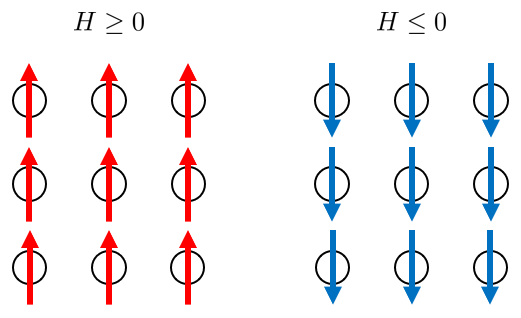
\includegraphics[height=5cm]{image/絶対零度スピン配位.png}
    \caption{絶対零度でのイジングモデルの基底状態.$H>0$のときはスピンはすべて上向きになり,$H<0$のときはスピンがすべて下向きになる$H=0$のときは,これら両方の状態が基底状態になる. \label{絶対零度スピン配位}}
  \end{center}
\end{figure}
これに基づいて,絶対零度での磁化のふるまいを見てみる.すべてのスピンが$+1$の状態での磁化は$\mu_0$,すべてのスピンが$-1$の状態での磁化は$-\mu_0$なので,
\begin{equation}
  m_L(\infty, H) =
  \begin{cases}
    -\mu_0, & H \leq 0 \text{のとき} \\
    \mu_0,  & H \geq 0 \text{のとき}
  \end{cases}
\end{equation}
とわかる.(図\ref{絶対零度磁化})
\begin{figure}[h]
  \begin{center}
    \begin{tikzpicture}[scale=1]
      \draw[->,>=stealth,semithick](-3,0)--(3,0)node[below]{$H$};%x軸
      \draw[->,>=stealth,semithick](0,-2.5)--(0,2.5)node[above]{$m(\infty, H)$};%y軸
      \draw[draw=magenta,thick,domain=0:3] plot(\x,2);
      \draw[draw=magenta,thick,domain=-3:0] plot(\x,-2);
      \draw (0,0) node[below left]{0}; %原点
      \draw (0,2) node[left]{$\mu_0$};
      \draw (0,-2) node[right]{$-\mu_0$};
    \end{tikzpicture}
    \caption{絶対零度でのイジングモデルの磁化のふるまい.$H=0$を境に,$-\mu_0$から$\mu_0$に不連続に変化する.\label{絶対零度磁化}}
  \end{center}
\end{figure}
つまり,磁化は$H$の関数として不連続である.もちろん,これはエネルギーを最小化する状態が入れ替わったことの単純な反映にすぎない.これに対して,同じような不連続性が$0$でない温度で見られるかどうかは,本質的に難しい問題である.

\subsection{無限体積の極限}
有限温度での相転移や臨界現象を調べるには,自由エネルギー$f_L(\beta, H)$や磁化$m_L(\beta, H)$といった物理量を計算し,それらの振る舞いを見ればよいと思える.しかし,このとき格子サイズ$L$はどの程度の大きさにとればよいのか?.実は格子サイズが有限である場合,相転移を起こさないことが示せる.ここではこれを証明する.\par
まず,格子サイズ$L$が任意の有限な整数とする.このとき,式(\ref{自由エネルギー})の形から明らかなように自由エネルギー$f_L(\beta, H)$は$\beta, H$について何度も微分できる.よって,磁化$m_L(\sigma, H)$は$H$の連続関数であることがわかる.そして,系の対称性を考える.あるスピン配位$(\sigma_1,\dots,\sigma_N)$が与えられたとき,これらすべてのスピンを反転させた新しいスピン配位を$(\tilde{\sigma}_1,\dots,\tilde{\sigma}_N)$で定義する.つまり,すべての$i$に対して$\tilde{\sigma}_i := -\sigma_i$とするということである.このとき,エネルギーの表式(\ref{イジングエネルギー})をスピン反転した変数を使って書き直せば,$\tilde{\sigma}_i \tilde{\sigma}_j = \sigma_i \sigma_j$が成り立つことを使って
\begin{equation}
  E_{(\sigma_1,\dots,\sigma_N)} = -J \sum_{\langle i,j \rangle} \tilde{\sigma}_i \tilde{\sigma}_j -h \sum_{i=1}^{N} \tilde{\sigma}_i
\end{equation}
のように,磁場を反転させた,元のエネルギーと同じ表式が得られる.つまり,すべてのスピンを反転させることは,磁場を反転させることと等価ということである.すべての$(\sigma_1,\dots,\sigma_N)$について足し上げることは,すべての$(\tilde{\sigma}_1,\dots,\tilde{\sigma}_N)$について足し上げることと同じなので,分配関数の表式(\ref{イジング分配関数})を,
\begin{align}
  Z_L(\beta, H)
   & = \sum_{(\tilde{\sigma}_1,\dots,\tilde{\sigma}_N)} \exp{[-\beta E_{(\sigma_1,\dots,\sigma_N)}]} \notag                                                                                               \\
   & = \sum_{(\tilde{\sigma}_1,\dots,\tilde{\sigma}_N)} \exp{\left[ \beta\left( J \sum_{\langle i,j \rangle} \tilde{\sigma}_i \tilde{\sigma}_j -H \sum_{i=1}^{N} \tilde{\sigma}_i \right) \right]} \notag \\
   & = \sum_{(\sigma_1,\dots,\sigma_N)} \exp{\left[ \beta\left( J \sum_{\langle i,j \rangle} \sigma_i \sigma_j -H \sum_{i=1}^{N} \sigma_i \right) \right]} \notag                                         \\
   & = Z_L(\beta, -H)
\end{align}
となり,磁場を反転させても分配関数は変わらないという結果になる.自由エネルギーの定義である式(\ref{自由エネルギー})より
\begin{equation}
  f_L(\beta, H) = f_L(\beta, -H)
\end{equation}
という自由エネルギーの対称性が示せる.さらに磁化は式(\ref{磁化と自由エネルギーの関係式})より,$f_L(\beta, H)$の$H$微分で書けるので,
\begin{equation}
  m_L(\beta, H) = -m_L(\beta, -H) \label{磁化反対称性}
\end{equation}
のように書け,磁化は磁場の反転について反対称になることがわかる.\par
$f_L(\beta, H)$が微分可能なので,$m_L(\beta, H)$はすべての$\beta, H$において定義されている.よって式(\ref{磁化反対称性})で$H=0$とすれば,$m_L(\beta, 0) = -m_L(\beta, 0)$となり,$m_L(\beta, 0)=0$が得られる.したがって,有限系では$0\leq \beta < \infty$の任意の逆温度$\beta$で磁化がゼロになり,相転移を示さないことがわかる.

\section{一次元イジング模型}
一次元のイジング模型を考える.ハミルトニアンは
\begin{equation}
  H = -J \sum_{i=1}^N \sigma_i \sigma_j - h \sum_{i=1}^N \sigma_i \label{一次元イジングエネルギー}
\end{equation}
なり,周期的境界条件$\sigma_{N+1} = \sigma_{1}$を課す.分配関数は
\begin{equation}
  Z = \sum_{(\sigma_i,\dots,\sigma_N)} \exp{\left[ \beta J \sum_{i=1}^N \sigma_i \sigma_j + \beta h \sum_{i=1}^N \sigma_i \right]} \label{一次元イジング分配関数}
\end{equation}
となる.ここで,次のような対称行列$\mathrm{T}$を定義する.
\begin{equation}
  (\mathrm{T})_{\sigma_i, \sigma_{i+1}} = \exp{\left[ \beta J \sigma_i \sigma_{i+1} + \frac{\beta h}{2}(\sigma_i + \sigma_{i+1}) \right]},
\end{equation}
\begin{equation}
  \mathrm{T} = \begin{pmatrix}
    (\mathrm{T})_{1,1}  & (\mathrm{T})_{1,-1}  \\
    (\mathrm{T})_{-1,1} & (\mathrm{T})_{-1,-1}
  \end{pmatrix}=
  \begin{pmatrix}
    e^{\beta J + \beta h} & e^{-\beta J}          \\
    e^{-\beta J}          & e^{\beta J - \beta h}
  \end{pmatrix}
\end{equation}
このようにすることで,分配関数(\ref{一次元イジング分配関数})を
\begin{align}
  Z
   & = \sum_{(\sigma_i,\dots,\sigma_N)} (\mathrm{T})_{\sigma_1, \sigma_2} (\mathrm{T})_{\sigma_2, \sigma_3} \cdots (\mathrm{T})_{\sigma_N, \sigma_1} \notag \\
   & = \sum_{(\sigma_i,\dots,\sigma_N)} \prod_{i = 1}^N (\mathrm{T})_{\sigma_i, \sigma_{i+1}}
\end{align}
を書くことができる.行列の積の定義より,
\begin{equation}
  \sum_{\sigma_k = \pm{1}}(\mathrm{T}^n)_{\sigma_i, \sigma_k}(\mathrm{T}^m)_{\sigma_k, \sigma_j}
  = (\mathrm{T}^{n+m})_{\sigma_i, \sigma_j}
\end{equation}
であることを用いると,分配関数は
\begin{align}
  Z
   & = \sum_{\sigma_1 = \pm{1}}\sum_{\sigma_2 = \pm{1}} \cdots \sum_{\sigma_N = \pm{1}} (\mathrm{T})_{\sigma_1, \sigma_2} (\mathrm{T})_{\sigma_2, \sigma_3} \cdots (\mathrm{T})_{\sigma_N, \sigma_1} \notag   \\
   & = \sum_{\sigma_1 = \pm{1}}\sum_{\sigma_3 = \pm{1}} \cdots \sum_{\sigma_N = \pm{1}} (\mathrm{T}^2)_{\sigma_1, \sigma_3} (\mathrm{T})_{\sigma_3, \sigma_4} \cdots (\mathrm{T})_{\sigma_N, \sigma_1} \notag \\
   & = \sum_{\sigma_1 = \pm{1}}\sum_{\sigma_4 = \pm{1}} \cdots \sum_{\sigma_N = \pm{1}} (\mathrm{T}^3)_{\sigma_1, \sigma_4} (\mathrm{T})_{\sigma_4, \sigma_5} \cdots (\mathrm{T})_{\sigma_N, \sigma_1} \notag \\
   & = \cdots \notag                                                                                                                                                                                          \\
   & = \sum_{\sigma_1 = \pm{1}} (\mathrm{T}^N)_{\sigma_1, \sigma_1} \notag                                                                                                                                    \\
   & = \mathrm{Tr}\left[ \mathrm{T}^N \right] \label{1Dイジング分配関数トレース}
\end{align}
と表すことができる.対称行列$\mathrm{T}$は,スピン間の相互作用を次々と伝える役割を果たしているため,転送行列(transfer matrix)と呼ばれる.\par
分配関数(\ref{1Dイジング分配関数トレース})は,初等的な線形代数の知識で計算することができる.実対称であるため,転送行列$\mathrm{T}$は適当な直行行列$\mathrm{O}$を用いて,
\begin{equation}
  \mathrm{O}^{-1} \mathrm{T} \mathrm{O} =
  \begin{pmatrix}
    \lambda_{+} & 0           \\
    0           & \lambda_{-}
  \end{pmatrix}
\end{equation}
と対角化できる.転送行列$\mathrm{T}$の固有値は
\begin{equation}
  \lambda_{\pm{1}}
  = e^{\beta} \left\{ \cosh{\beta h} \pm{\sqrt{(\sinh{\beta h})^2 + e^{-4\beta J}}} \right\}
\end{equation}
より,(\ref{1Dイジング分配関数トレース})はさらに
\begin{align}
  Z
   & = \mathrm{Tr} \left[ \left\{ \mathrm{O}
  \begin{pmatrix}
      \lambda_{+} & 0           \\
      0           & \lambda_{-}
    \end{pmatrix} \mathrm{O}^{-1} \right\}^N \right] \notag   \\
   & = \mathrm{Tr} \left[
  \begin{pmatrix}
      \lambda_{+} & 0           \\
      0           & \lambda_{-}
    \end{pmatrix}^N \right] \notag                            \\
   & = (\lambda_{+})^N + (\lambda_{-})^N \label{1Dイジング分配関数}
\end{align}
と表すことができる.\par
(\ref{1Dイジング分配関数})より,スピン一つあたりの自由エネルギー$f$は
\begin{align}
  f
   & = -\frac{1}{\beta L} \ln{Z} \notag                                                                                              \\
   & = -\frac{1}{\beta L} \ln{(\lambda_{+})^N + (\lambda_{-})^N} \notag                                                              \\
   & = -\frac{1}{\beta} \ln{\lambda_{+}} - \frac{1}{\beta L} \left\{ 1 + \left( \frac{\lambda_{-}}{\lambda_{+}} \right)^{L} \right\}
\end{align}
と表すことができる.ここで,$\lambda{-}/\lambda_{+}<1$に注意して,$L \nearrow \infty$とすると,
\begin{align}
  f
   & = \lim_{L \nearrow \infty} f = -\frac{1}{\beta} \ln{\lambda_{+}} \notag                                                   \\
   & = -\frac{1}{\beta} \ln{e^{\beta} \left\{ \cosh{\beta h} \pm{\sqrt{(\sinh{\beta h})^2 + e^{-4\beta J}}}\right\}} \notag    \\
   & = -1 -\frac{1}{\beta} \ln{\left\{\cosh{\beta h} \pm{\sqrt{(\sinh{\beta h})^2 + e^{-4\beta J}}}\right\}} \label{1D自由エネルギー}
\end{align}
となり,無限体積極限での自由エネルギーを厳密に計算することができる.\par
自由エネルギーの表式(\ref{1D自由エネルギー})から,磁化を計算すると,
\begin{align}
  m(\beta, h)
   & = -\frac{\partial}{\partial h} f(\beta, h) \notag                                                                                                                                                   \\
   & = \frac{\partial}{\partial (\beta h)} \ln{\left\{ \cosh{\beta h} + \sqrt{(\sinh{\beta h})^2 + e^{-4\beta J}} \right\}} \notag                                                                       \\
   & = \frac{1}{\cosh{\beta h} + \sqrt{(\sinh{\beta h})^2 + e^{-4\beta J}}} \frac{\partial}{\partial (\beta h)}\left\{ \cosh{\beta h} + \sqrt{(\sinh{\beta h})^2 + e^{-4\beta J}} \right\} \notag        \\
   & =  \frac{1}{\cosh{\beta h} + \sqrt{(\sinh{\beta h})^2 + e^{-4\beta J}}} \left\{ \sinh{\beta h} + \frac{2\sinh{\beta h} \cosh{\beta h}}{2 \sqrt{(\sinh{\beta h})^2 + e^{-4\beta J}}} \right\} \notag \\
   & = \frac{\sinh{\beta h}}{\sqrt{(\sinh{\beta h})^2 + e^{-4\beta J}}}
\end{align}
となる.これは明らかに$\beta$と$h$について連続な関数である.特に$h=0$のとすれば$m(\beta, 0) = 0$となる.つまり,有限温度の一次元イジング模型での自発磁化は$0$であり,この系は相転移を示さないことがわかる.\par
さらに,この結果を使って磁化率$\chi(\beta)$を求めると,
\begin{align}
  \chi(\beta)
   & = \left.\frac{\partial}{\partial h} m(\beta, h)\right|_{h=0} \notag                                                                                                                                       \\
   & = \left.\frac{\partial}{\partial h} \frac{\sinh{\beta h}}{\sqrt{(\sinh{\beta h})^2 + e^{-4\beta J}}}\right|_{h=0} \notag                                                                                  \\
   & = \beta \left.\frac{\partial}{\partial (\beta h)} \frac{\sinh{\beta h}}{\sqrt{(\sinh{\beta h})^2 + e^{-4\beta J}}}\right|_{h=0} \notag                                                                    \\
   & = \beta \left.\left[ \frac{\cosh{\beta h}}{\sqrt{(\sinh{\beta h})^2 + e^{-4\beta J}}} +\frac{(\sinh{\beta h})^2 \cosh{\beta h}}{\{(\sinh{\beta h})^2 + e^{-4\beta J}\}^{3/2}} \right]\right|_{h=0} \notag \\
   & = \beta e^{2\beta J}
\end{align}
となる.$\beta J \ll 1$が成り立つ高温領域では,$\chi(\beta) \simeq \beta$となり,相互作用のない場合の振る舞い(キュリーの法則)が成り立つ.一方,低温に向かい$\beta \rightarrow \infty$となると,相互作用のない場合の磁化率との比$e^{2\beta J}$は限りなく大きくなる.これは,低温で無限個のスピンが互いにそろい合おうとすることの現れとみることができる.\par

% \section{イジング模型の平均場近似}




\begin{figure}[htbp]
  \begin{minipage}[b]{0.45\linewidth}
    \centering
    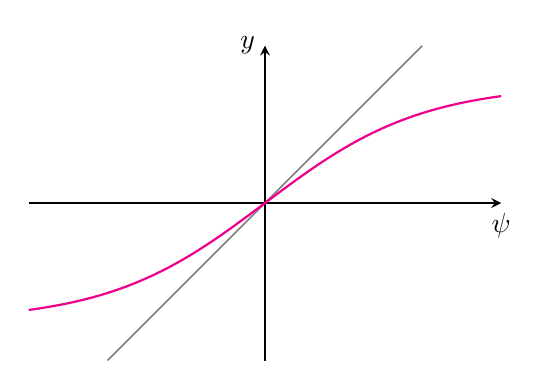
\begin{tikzpicture}[scale=1,samples=300]
      \draw[->,>=stealth,semithick](-3,0)--(3,0)node[below]{$\psi$};%x軸
      \draw[->,>=stealth,semithick](0,-2)--(0,2)node[left]{$y$};%y軸
      \draw[draw=gray,semithick,domain=-2:2] plot(\x,\x);
      \draw[draw=magenta,thick,domain=-3:3] plot(\x,{1.5*tanh(0.5*\x)});
    \end{tikzpicture}
    \subcaption{$\beta zJ \leq 1$}
  \end{minipage}
  \begin{minipage}[b]{0.45\linewidth}
    \centering
    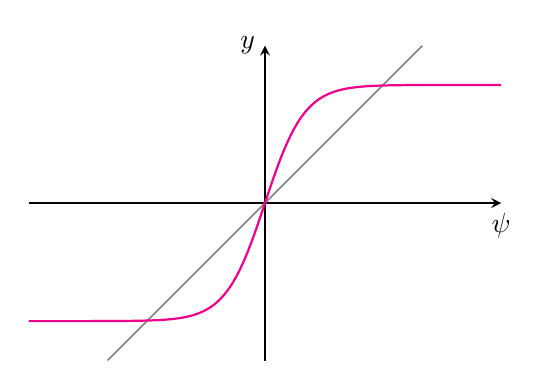
\begin{tikzpicture}[scale=1,samples=300]
      \draw[->,>=stealth,semithick](-3,0)--(3,0)node[below]{$\psi$};%x軸
      \draw[->,>=stealth,semithick](0,-2)--(0,2)node[left]{$y$};%y軸
      \draw[draw=gray,semithick,domain=-2:2] plot(\x,\x);
      \draw[draw=magenta,thick,domain=-3:3] plot(\x,{1.5*tanh(2*\x)});
    \end{tikzpicture}
    \subcaption{$\beta zJ > 1$}
  \end{minipage}
  \caption{$h=0$での自己整合方程式$\psi = \tanh{(\beta ZJ\psi)}$}
\end{figure}

\section{二次元イジング模型}
\section{二次元イジング模型の厳密解の計算}
二次元イジング模型の厳密解はOnsagerによって求められた.Onsagerは,転送行列を対角化することで磁場のないときの自由エネルギーを求め,比熱をある温度で発散することを示した.いくつかの解法があるが,ここでは,高温展開を用いた解法を説明する.高温展開は,温度が高いとして自由エネルギーを$\beta J$のべきで展開する方法である.十分高温であれば,その展開を数項で打ち切って自由エネルギーの近似値とする.計算が比較的簡単なため,汎用的な手法として用いられているが,近似の正当性に十分に注意する必要がある.この近似のみを用いて相転移を調べることはできない.有限項の和から特異性が生じることはないからである.本節では,無限和を計算することにより厳密解を求め,特異性が生じることを示す.\par
\subsection{高温展開}
$h=0$の場合に高温展開を行う.二次元イジング模型の分配関数は
\begin{equation}
  Z = \mathrm{Tr}\prod_{\langle i, j \rangle} \exp{(\beta J \sigma_i \sigma_j)}
\end{equation}
と書ける.積はスピンの最近近接についてとる.スピン変数に関する恒等式
\begin{align}
  e^{x\sigma_i \sigma_j}
   & = \frac{e^x + e^{-x}}{2} + \sigma_i \sigma_j \frac{e^x + e^{-x}}{2} \notag \\
   & = \cosh{x} + \sigma_i \sigma_j \sinh{x}
\end{align}
を用いれば,
\begin{align}
  Z
   & = \mathrm{Tr}\prod_{\langle i, j \rangle}(\cosh{\beta J} + \sigma_i \sigma_j \sinh{\beta J}) \notag                \\
   & = (\cosh{\beta J})^{N_B}\mathrm{Tr}\prod_{\langle i, j \rangle}(1 + \sigma_i \sigma_j \tanh{\beta J}) \label{分配関数}
\end{align}
と書ける.$N_B$は最近接の数を表す.$v = \tanh{\beta J}$は有限温度で$1$より有限温度で$1$より小さい非負の量なので,(\ref{分配関数})を$v$について次のように展開する.
\begin{equation}
  \prod_{\langle i, j \rangle}(1 + v \sigma_i \sigma_j)
  = 1 + v \sum_{\langle i, j \rangle} \sigma_i \sigma_j
  + v^2 \sum_{\langle i, j \rangle, \langle k, l \rangle} \sigma_i \sigma_j \sigma_k \sigma_l + \cdots
\end{equation}
ここで,$\langle i, j \rangle \neq \langle k, l \rangle$である.

\begin{equation}
  v\sigma_i \sigma_j \longleftrightarrow
  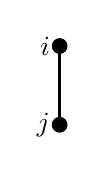
\begin{tikzpicture}[baseline={([yshift=-.5ex]current bounding box.center)}]
    \draw[very thick](0,0)--(0,-1);
    \fill(0,0)circle(0.1)node[left]{$i$};
    \fill(0,-1)circle(0.1)node[left]{$j$};
  \end{tikzpicture}
\end{equation}

\begin{equation}
  v^2\sigma_i \sigma_j \sigma_k \sigma_l \longleftrightarrow
  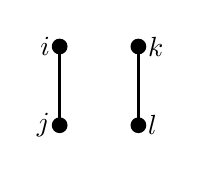
\begin{tikzpicture}[baseline={([yshift=-.5ex]current bounding box.center)}]
    \draw[very thick](0,0)--(0,-1);
    \draw[very thick](1,0)--(1,-1);
    \fill(0,0)circle(0.1)node[left]{$i$};
    \fill(0,-1)circle(0.1)node[left]{$j$};
    \fill(1,0)circle(0.1)node[right]{$k$};
    \fill(1,-1)circle(0.1)node[right]{$l$};
  \end{tikzpicture}, \ \ \
  v^2\sigma_i \sigma_j^2 \sigma_k \longleftrightarrow
  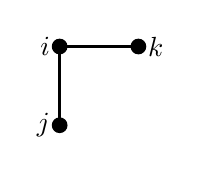
\begin{tikzpicture}[baseline={([yshift=-.5ex]current bounding box.center)}]
    \draw[very thick](0,0)--(0,-1);
    \draw[very thick](0,0)--(1,0);
    \fill(0,0)circle(0.1)node[left]{$i$};
    \fill(0,-1)circle(0.1)node[left]{$j$};
    \fill(1,0)circle(0.1)node[right]{$k$};
  \end{tikzpicture}
\end{equation}

\begin{equation}
  Z = (\cosh{\beta J})^{N_B}\mathrm{Tr}
  \left[
    1 + \sum
    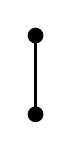
\begin{tikzpicture}[baseline={([yshift=-.5ex]current bounding box.center)}]
      \draw[very thick](0,0)--(0,-1);
      \fill(0,0)circle(0.1);
      \fill(0,-1)circle(0.1);
    \end{tikzpicture}
    + \sum
    \left(
    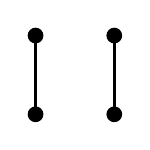
\begin{tikzpicture}[baseline={([yshift=-.5ex]current bounding box.center)}]
      \draw[very thick](0,0)--(0,-1);
      \draw[very thick](1,0)--(1,-1);
      \fill(0,0)circle(0.1);
      \fill(0,-1)circle(0.1);
      \fill(1,0)circle(0.1);
      \fill(1,-1)circle(0.1);
    \end{tikzpicture} +
    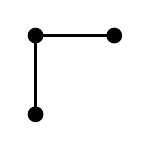
\begin{tikzpicture}[baseline={([yshift=-.5ex]current bounding box.center)}]
      \draw[very thick](0,0)--(0,-1);
      \draw[very thick](0,0)--(1,0);
      \fill(0,0)circle(0.1);
      \fill(0,-1)circle(0.1);
      \fill(1,0)circle(0.1);
    \end{tikzpicture}
    \right) + \cdots
    \right]
\end{equation}

\subsection{行列を用いた定式化}
2次元イジング模型の厳密解に向けた前段階として,行列の観点で2次元イジングモデルの定式化を行う.$n$行$n$列の正方格子上にある$N=n^2$個のスピンを考える.そして,周期的境界条件を課す.\par
スピン座標の$\alpha$列にあるスピンをまとめて次のように表す.
\begin{equation}
  \mu_{\alpha}
  \equiv \{\sigma_1, \sigma_2, \dots, \sigma_n\}
\end{equation}
境界条件より,
\begin{align}
  \mu_{n+1}    & = \mu_1    \\
  \sigma_{n+1} & = \sigma_1
\end{align}
が成り立つ.また,配位全体を$\{\mu_1, \dots, \mu_n\}$と表す.仮定より,$\alpha$列のスピンと相互作用するのは$(\alpha-1)$列と$(\alpha+1)$列である.ここで,$\alpha$列と$\alpha+1$列との相互作用エネルギーを$E(\mu_{\alpha}, \mu_{\alpha+1})$,$\alpha$列のスピン内でのスピン同士の相互作用エネルギーと磁場との相互作用エネルギーを$E(\mu_{\alpha})$とすると,それぞれ次のように書ける.
\begin{align}
  E(\mu, \mu')
   & = -\epsilon \sum_{k=1}^n s_k s'_k                         \\
  E(\mu)
   & = -\epsilon \sum_{k=1}^n s_k s_{k+1} - H \sum_{k=1}^n s_k
\end{align}
ここで,$\mu$と$\mu'$はそれぞれ,隣り合った列のスピン座標の集まりである.
\begin{align}
  \mu  & \equiv \{s_1, \dots, s_n \} \notag \\
  \mu' & \equiv \{s'_1, \dots, s'_n \}
  \label{イジングエネルギー2}
\end{align}
配位$\{\mu_1, \dots, \mu_n\}$における全エネルギーは
\begin{equation}
  E_t\{\mu_1, \dots, \mu_n \}
  = \sum_{\alpha=1}^n [E(\mu_{\alpha}, \mu_{\alpha+1}) + E(\mu_{\alpha})]
\end{equation}
となり,分配関数は
\begin{equation}
  Z(H,T)
  = \sum_{\mu_1} \cdots \sum_{\mu_n} \exp{\left\{ -\beta \sum_{\alpha=1}^n [E(\mu_{\alpha}, \mu_{\alpha+1}) + E(\mu_{\alpha})] \right\}}
\end{equation}
となる.\par
ここで,次のように行列要素が定義された,$2^n \times 2^n$行列$\mathrm{P}$を考える.
\begin{equation}
  \bra{\mu} \mathrm{P} \ket{\mu'} \equiv e^{-\beta [E(\mu_{\alpha}, \mu_{\alpha+1}) + E(\mu_{\alpha})]}
  \label{行列要素}
\end{equation}
これを用いると分配関数は
\begin{align}
  Z(H,T)
   & = \sum_{\mu_1} \cdots \sum_{\mu_n} \bra{\mu_1} \mathrm{P} \ket{\mu_2}\bra{\mu_2} \mathrm{P} \ket{\mu_3}\cdots\bra{\mu_n} \mathrm{P} \ket{\mu_1} \\
   & = \sum_{\mu_1}\bra{\mu_1} \mathrm{P}^n \ket{\mu_1} = \mathrm{Tr} \ \mathrm{P}^n
\end{align}
と$\mathrm{P}^n$のトレースで表せることがわかる.行列のトレースは行列の表現から独立しているため,上式のトレースは,以下のような対角化された$\mathrm{P}$で評価しても結果に影響を与えない.
\begin{equation}
  \mathrm{P} = \begin{bmatrix}
    \lambda_1 &           &        &               \\
              & \lambda_2 &        &               \\
              &           & \ddots &               \\
              &           &        & \lambda_{2^n} \\
  \end{bmatrix}
\end{equation}
ここで,$\lambda_1, \lambda_2, \dots, \lambda_{2^n}$は$\mathrm{P}$の固有値である.$\mathrm{P}^n$もまた対角行列であり,対角成分は$(\lambda_1)^n, (\lambda_2)^n, \dots, (\lambda_{2^n})^n$である.したがって,分配関数は
\begin{equation}
  Z(H,T)
  = \sum_{\alpha=1}^{2^n} (\lambda_\alpha)^n
\end{equation}
で表される.$E(\mu, \mu')$と$E(\mu)$は$n$のオーダーであるため,式(\ref{行列要素})の形式から,$n$が大きい場合,$\mathrm{P}$の固有値は一般に$e^n$のオーダーであることが予想される.$\lambda_{\text{max}}$を$\mathrm{P}$の最大固有値とすると,
\begin{equation}
  \lim_{n \rightarrow \infty} \frac{1}{n} \ln{\lambda}_{\text{max}}
  = \text{finite number}
  \label{最大固有値有限}
\end{equation}
と予想される.そして,もしこれが正しく,すべての固有値$\lambda_{\alpha}$が正ならば,
\begin{equation}
  (\lambda_{\text{max}})^n \leq Z \leq 2^n (\lambda_{\max})^n
\end{equation}
もしくは
\begin{equation}
  \frac{1}{n}\ln{\lambda_{\text{max}}}
  \leq \frac{1}{n^2}\ln{Z}
  \leq \frac{1}{n}\ln{\lambda_{\text{max}}} + \frac{1}{n} \ln{2}
\end{equation}
となる.したがって,はさみうちの原理より,
\begin{equation}
  \lim_{N \rightarrow \infty} \frac{1}{N} \ln{Z}
  = \lim_{n \rightarrow \infty} \frac{1}{n} \ln{\lambda_{\text{max}}}
  \label{n極限}
\end{equation}
か成り立つことがわかる.ここで,$N=n^2$.式(\ref{最大固有値有限}) が真であり,すべての固有値$\lambda_{\alpha}$が正であることがわかる.したがって,$P$の最大の固有値を見つけるだけで十分である.このセクションの残りの部分は,$P$の明示的な表現の説明に当てられる.

\subsection{行列$\mathrm{P}$}
式(\ref{行列要素})と式(\ref{イジングエネルギー2})から我々は$\mathrm{P}$の行列要素を
\begin{align}
  \bra{s_1,\dots,s_n}\mathrm{P}\ket{s'_1,\dots,s'_n}
   & = e^{-\beta[E(\mu, \mu') + E(\mu)]} \notag                                                        \\
   & = e^{\beta \sum_{k=1}^{n}} \left( \epsilon s_k s'_k + \epsilon s_k s_{k+1} + H s_k \right) \notag \\
   & = \prod_{k=1}^n e^{\beta H s_k} e^{\beta \epsilon s_k s_{k+1}} e^{\beta \epsilon s_k s'_k}
\end{align}
のように得た.ここで,$2^n \times 2^n$の3つの行列$V'_1, V_2, V_3$を定義する.それぞれ行列要素は次のように与える.
\begin{align}
  \bra{s_1,\dots,s_n}V'_1\ket{s'_1,\dots,s'_n}
   & \equiv \prod_{k=1}^n e^{\beta \epsilon s_k s'_k} \label{V1}                                 \\
  \bra{s_1,\dots,s_n}V_2\ket{s'_1,\dots,s'_n}
   & \equiv \delta_{s_1 s'_1}\dots\delta_{s_n s'_n} \prod_{k=1}^n e^{\beta \epsilon s_k s_{k+1}} \\
  \bra{s_1,\dots,s_n}V_3\ket{s'_1,\dots,s'_n}
   & \equiv \delta_{s_1 s'_1}\dots\delta_{s_n s'_n} \prod_{k=1}^n e^{\beta \epsilon H s_k}       \\
\end{align}
ここで,$\delta_{ss'}$はクロネッカーのデルタ記号である.したがって,この表現では$V_2$と$V_3$は対角行列になる.それは簡単に示せる.
\begin{equation}
  \mathrm{P} = V_3 V_2 V'_1
\end{equation}
行列乗算の通常の意味で,つまり
\begin{align*}
  & \bra{s_1,\dots,s_n}\mathrm{V}_3\mathrm{V}_2\mathrm{V}'_1\ket{s'_1,\dots,s'_n}                                                            \\
  & = \sum_{s''_1, \dots, s''_n} \sum_{s'''_1, \dots, s'''_n} \bra{s_1,\dots,s_n}\mathrm{V}_3\ket{s''_1,\dots,s''_n} \bra{s''_1,\dots,s''_n}\mathrm{V}_2\ket{s'''_1,\dots,s'''_n}       \\
  & \times \bra{s'''_1,\dots,s'''_n}\mathrm{V}'_1\ket{s'_1,\dots,s'_n} \\
  & = \sum_{s''_1, \dots, s''_n} \sum_{s'''_1, \dots, s'''_n}
  \delta_{s_1s''_1} \cdots \delta_{s_ns''_n} \delta_{s''_1s'''_1} \cdots \delta_{s''_ns'''_n} \prod_{k =1}^{n} e^{\beta H s_k} e^{\beta \epsilon s''_k s'''_{k+1}} e^{\beta \epsilon s'''_k s'_k} \\
  & = \sum_{s''_1, \dots, s''_n} 
  \delta_{s_1s''_1} \cdots \delta_{s_ns''_n} \prod_{k =1}^{n} e^{\beta H s_k} e^{\beta \epsilon s''_k s''_{k+1}} e^{\beta \epsilon s''_k s'_k} \\
  & = \prod_{k =1}^{n} e^{\beta H s_k} e^{\beta \epsilon s_k s_{k+1}} e^{\beta \epsilon s_k s'_k}
\end{align*}

\subsection{行列の直積}
ここで,$\mathrm{V}_3, \mathrm{V}_2, \mathrm{V}'_1$による便利な方法を述べる前に,行列の積の概念を導入する.\par
$m \times m$の2つの行列$A, B$を考える.行列要素はそれぞれ,$\bra{i}A\ket{j}, \bra{i}B\ket{j}$である.$i, j$はそれぞれ$1, 2, \dots, m$の値をとる.このとき,直積$A \times B$は$m^2 \times m^2$の行列となり,行列要素は
\begin{equation}
  \bra{ii'}A \times B\ket{jj'}
  \equiv \bra{i} A \ket{j} \bra{i'} B \ket{j'}
\end{equation}
と定義する.3つ以上の行列の直積$A \times B \times \cdots \times C$にも拡張でき,行列要素は
\begin{equation}
  \bra{ii' \cdots i''} A \times B \times \cdots \times C \ket{jj' \cdots j''}
  \equiv \bra{i}A\ket{j} \bra{i'}B\ket{j'} \cdots \bra{i''}A\ket{j''}
\end{equation}
で表される.もし$AB$が通常の行列乗算のもとでの行列AとBの積を表すなら,次のようになる.
\begin{equation}
  (A \times B)(C \times D) = (AC) \times (BD)
\end{equation}
これは以下のように示せる.
\begin{align*}
  \bra{ii'} (A \times B)(C \times D) \ket{jj'}
   & = \sum_{kk'} \bra{ii'} A \times B \ket{kk'} \bra{kk'} C \times D \ket{jj'} \\
   & = \bra{i} AC \ket{j} \bra{i'} BD \ket{j'}                                  \\
   & = \bra{ii'} (AC) \times (BD) \ket{jj'}
  \label{直積公式}
\end{align*}
式(\ref{直積公式})を一般化した,以下の等式も成り立つ.
\begin{equation}
  (A \times B \times \cdots \times C) (D \times E \times \cdots \times F)
  = (AD) \times (BE) \times \cdots \times (CF)
\end{equation}

\subsection{スピン行列}
ここで,$\mathrm{V}'_1, \mathrm{V}_2, \mathrm{V}_3$を便利に表現できる特別な行列をいくつか紹介する.よく知られた3つの$2 \times 2$パウリスピン行列を$X, Y, Z$とする.
\begin{equation}
  X \equiv \begin{pmatrix}
    0 & 1 \\ 1 & 0
  \end{pmatrix}, \ \ \
  Y \equiv \begin{pmatrix}
    0 & -i \\ i & 0
  \end{pmatrix}, \ \ \
  Z \equiv \begin{pmatrix}
    1 & 0 \\ 0 & -1
  \end{pmatrix}
\end{equation}
これらパウリ行列は次の関係式を満たす.\par
\begin{equation*}
  X^2 = Y^2 = Z^2 = 1
\end{equation*}
\begin{equation}
  XY + YX = 0, \ \ YZ + ZY = 0, \ \ ZX + XZ = 0
  \label{スピン行列性質}
\end{equation}
\begin{equation*}
  XY = iZ, \ \ YZ = iX, \ \ ZX = iY
\end{equation*}
ここで,$2^n \times 2^n$行列$\mathrm{X}_{\alpha}, \mathrm{Y}_{\alpha}, \mathrm{Z}_{\alpha}$を定義する.
\begin{align}
  \mathrm{X}_{\alpha} \equiv 1 \times 1 \times \cdots \times \mathrm{X} \times \cdots \times 1 \notag \\
  \mathrm{Y}_{\alpha} \equiv 1 \times 1 \times \cdots \times \mathrm{Y} \times \cdots \times 1        \\
  \mathrm{Z}_{\alpha} \equiv 1 \times 1 \times \cdots \times \mathrm{Z} \times \cdots \times 1 \notag
\end{align}
$\alpha \neq \beta$のとき以下の関係式が成り立つ.
\begin{align}
   & [\mathrm{X}_{\alpha}, \mathrm{X}_{\beta}]
  = [\mathrm{Y}_{\alpha}, \mathrm{Y}_{\beta}]
  = [\mathrm{Z}_{\alpha}, \mathrm{Z}_{\beta}]
  = 0 \notag                                   \\
   & [\mathrm{X}_{\alpha}, \mathrm{Y}_{\beta}]
  = [\mathrm{X}_{\alpha}, \mathrm{Z}_{\beta}]
  = [\mathrm{Y}_{\alpha}, \mathrm{Z}_{\beta}]
  = 0
\end{align}
$2^n \times 2^n$行列$\mathrm{X}_{\alpha}, \mathrm{Y}_{\alpha}, \mathrm{Z}_{\alpha}$は(\ref{スピン行列性質})のすべての関係式を満たす.

\subsection{行列$\mathrm{V}'_1, \mathrm{V}_2, \mathrm{V}_3$}
式(\ref{V1})から,$\mathrm{V}'_1$が$n$個の同じ$2 \times 2$行列の直積で表せることがわかる.
\begin{equation}
  \mathrm{V}_1'=\bm{a} \times \bm{a} \times \cdots \times \bm{a}
\end{equation}
ここで,
\begin{equation}
  \bra{s}\bm{a} \ket{s'}
  =e^{\beta \epsilon s s'}
\end{equation}
である.したがって,
\begin{equation}
  \bm{a}=\left[\begin{array}{cc}
      e^{\beta \epsilon}  & e^{-\beta \epsilon} \\
      e^{-\beta \epsilon} & e^{\beta \epsilon}
    \end{array}\right]=e^{\beta \epsilon}+e^{-\beta \epsilon} X
    \label{a行列}
\end{equation}
である.ここで,$\alpha$と$\theta$を定数として
\begin{equation}
  \bm{a} 
  = \alpha e^{\theta X}
  = \alpha (\cosh{\theta} + X \sinh{\theta})
\end{equation}
として,式(\ref{a行列})と係数比較すれば,
\begin{equation}
  \begin{cases}
    e^{\beta \epsilon} = \alpha \cosh{\theta} \\
    e^{- \beta \epsilon} = \alpha \sinh{\theta}
  \end{cases}
\end{equation}
となり,これを解くことで
\begin{equation}
  \bm{a}
  =\sqrt{2 \sinh (2 \beta \epsilon)} e^{\theta X}, \quad
  \tanh \theta \equiv e^{-2 \beta \epsilon}
\end{equation}
である.したがって
\begin{equation}
  \mathrm{V}_1'=[2 \sinh (2 \beta \epsilon)]^{\frac{n}{2}} e^{\theta X} \otimes e^{\theta X} \otimes \cdots \otimes e^{\theta X}
\end{equation}
と表せる.ここで,
\begin{align}
  &e^{\theta X} \otimes e^{\theta X} \otimes \cdots \otimes e^{\theta X} \\
  &= (e^{\theta X} \otimes 1 \otimes \cdots \otimes 1) (1 \otimes e^{\theta X} \otimes \cdots \otimes 1) \cdots (1 \otimes 1 \otimes \cdots \otimes e^{\theta X}) \\
  &= e^{\theta \mathrm{X}_1} e^{\theta \mathrm{X}_2} \cdots e^{\theta \mathrm{X}_n} \\
  &= e^{\theta\left(\mathrm{X}_1+\mathrm{X}_2+\cdots+\mathrm{X}_n\right)}
\end{align}
と表せることを使う.2つ目の等式では$1 \otimes \cdots \otimes e^{\theta X} \otimes \cdots \otimes 1 = e^{\theta (1 \otimes \cdots \otimes X \otimes \cdots 1)}$を使った.これより,$\mathrm{V}'_1$は次のように書ける.
\begin{align}
  \mathrm{V}_1'
   & =[2 \sinh (2 \beta \epsilon)]^{\frac{n}{2}} \mathrm{~V}_1                               \\
  \mathrm{V}_1
   & =\prod_{\alpha=1}^n e^{\theta \mathrm{x}_{\alpha}}, \quad \tanh \theta \equiv e^{-2 \beta \epsilon}
\end{align}
同様な考えより,$\mathrm{V}_2, \mathrm{V}_3$に関しても,
\begin{align}
  \mathrm{V}_2
   & =\prod_{\alpha=1}^n e^{\beta \epsilon \mathbf{Z}_\alpha \mathbf{Z}_{\alpha+1}}                      \\
  \mathrm{~V}_3
   & =\prod_{\alpha=1}^n e^{\beta H \mathbf{Z}_\alpha} \quad, \quad \mathbf{Z}_{n+1} \equiv \mathbf{Z}_1
\end{align}
が示せる.したがって
\begin{equation}
  \mathrm{P}
  = [2 \sinh (2 \beta \epsilon)]^{\frac{n}{2}} \mathrm{V}_3 \mathrm{V}_2 \mathrm{V}_1
  \label{行列P最終形態}
\end{equation}
と表すことができる.$H=0$のとき,つまり$V_3 = 1$のとき,2次元イジング模型を完全に定式化できる.

\subsection{厳密解}
磁場がない場合,式(\ref{n極限})と式(\ref{行列P最終形態})は次のようになる.
\begin{equation}
  \lim_{N \rightarrow \infty} \frac{1}{N} \ln{Z(0, T)} 
  = \frac{1}{2} \ln{[2 \sinh{2 \beta \epsilon}]}
  + \lim_{n \rightarrow \infty} \frac{1}{n} \ln{\Lambda}
\end{equation}
ここで,$\Lambda$は$\mathrm{V} = \mathrm{V}_1 \mathrm{V}_2$の最大固有値である.また,$\mathrm{V}_1$は式(\ref{})で与えられ,$\mathrm{V}_1$は(\ref{})で与えられる.これらの式は,Vの固有値がすべて正で,$\lim_{n \rightarrow \infty} n^{-1}\ln{\Lambda}$が存在する場合に成り立つ.我々の主な仕事は行列$\mathrm{V}$を対角化することである.


\chapter{機械学習と深層学習}
ここでは,イジングモデルに対して機械学習,深層学習による手法を応用する上で必要となる機械学習と深層学習の基礎知識について説明する.
\section{機械学習とは}
機械学習(machine learning)とは,人間がこなすような学習や知的作業を計算機に実行させるためのアプローチの研究,あるいはその手法そのもののことを意味する.機械学習では,知識を人間が直接アルゴリズムに具体的に書き込んだり教え込んだりせず,データという具体例の集まりから計算機に自動的に学ばせるという方法をとる.\par
機械学習の定義としてT. M. ミッチェル(Tom Michael Mitchell)の書籍\cite{Tom1997Machine}で書かれている定義が有名である.それは
\begin{quote}
  "コンピュータプログラムが,ある種のタスクTとパフォーマンス評価尺度Pにおいて,経験Eから学習するとは,タスクTにおけるその性能をPによって評価した際に,経験Eによってそれが改善されている場合である."
  \hfill T. M. ミッチェル
\end{quote}
である.ここで,タスクTとは解きたい問題のこと,パフォーマンス評価尺度Pは精度,誤差率などの評価指標のこと,経験Eはデータセットのことを指す.\par
機械学習では,何かしらのモデルを構築する必要がある.このモデルというのは,なにかしらの入力が与えられたときに出力を返すものであり,その正体は多数のパラメータを持った非線形関数$f_{\bm{\theta}}(\bm{x}), \ \bm{\theta} = \{ \theta_1, \theta_2, \theta_3, \cdots \}$である.
\begin{figure}[b]
  \begin{center}
    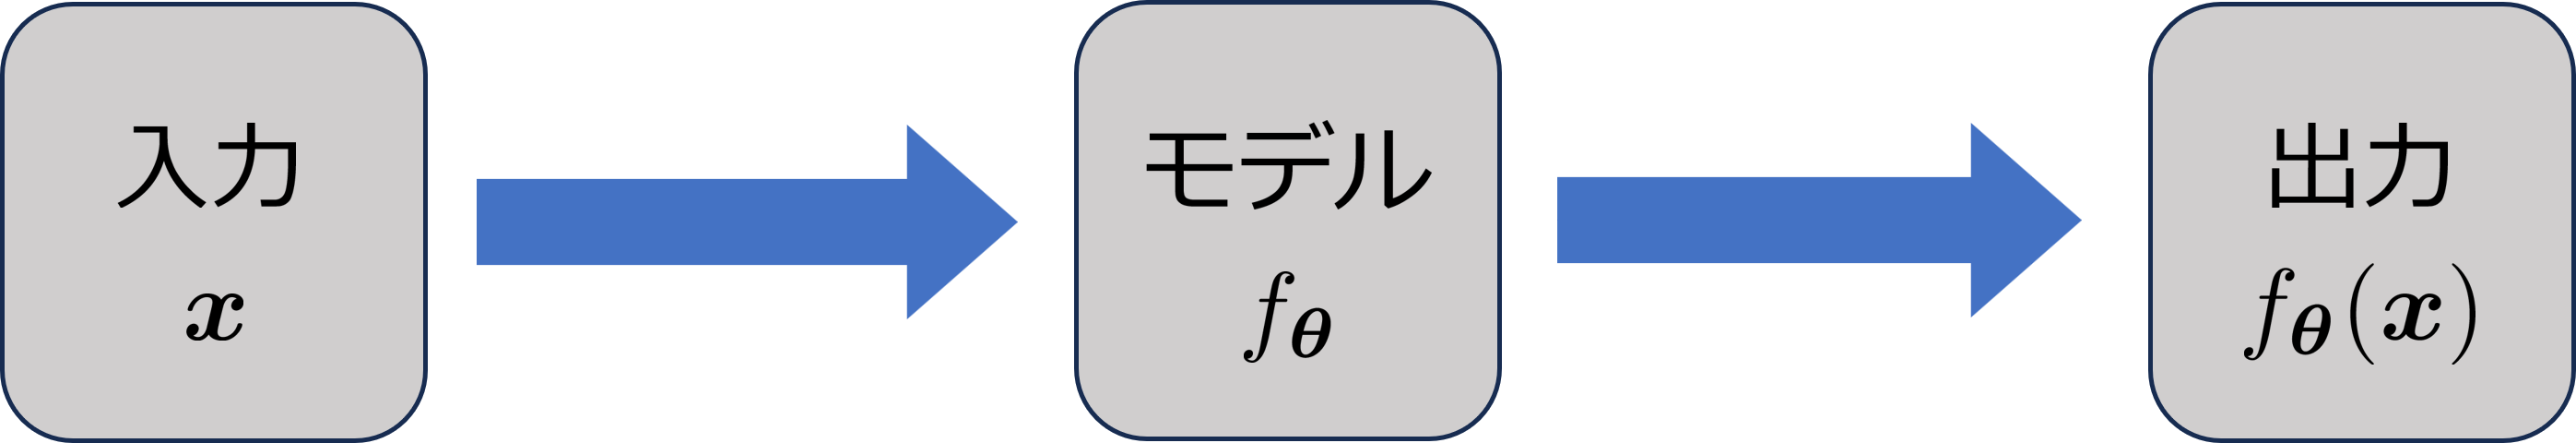
\includegraphics[height=1.5cm]{image/モデル概略図.png}
    \caption{モデルの概略図}
  \end{center}
\end{figure}
このパラメータの値は最初はランダムに初期化されており,入力を与えると出力が返ってくるが,このときの出力結果は本来出力してほしい正解の値からは外れた値が帰ってくる.そこで,出力と正解の誤差を測るような評価基準を決めておき,算出された評価結果を良くするようにモデルのパラメータを更新してあげることによってモデルを改善していく.この一連の流れを繰り返し行うことで,モデルを改善して,正解に近い出力結果を得られるモデルを作成すること機械学習とよぶ.ここで注目してほしいのは,機械学習ではモデルの改善を機械に行わせているという点である.\par
\begin{figure}[t]
  \begin{center}
    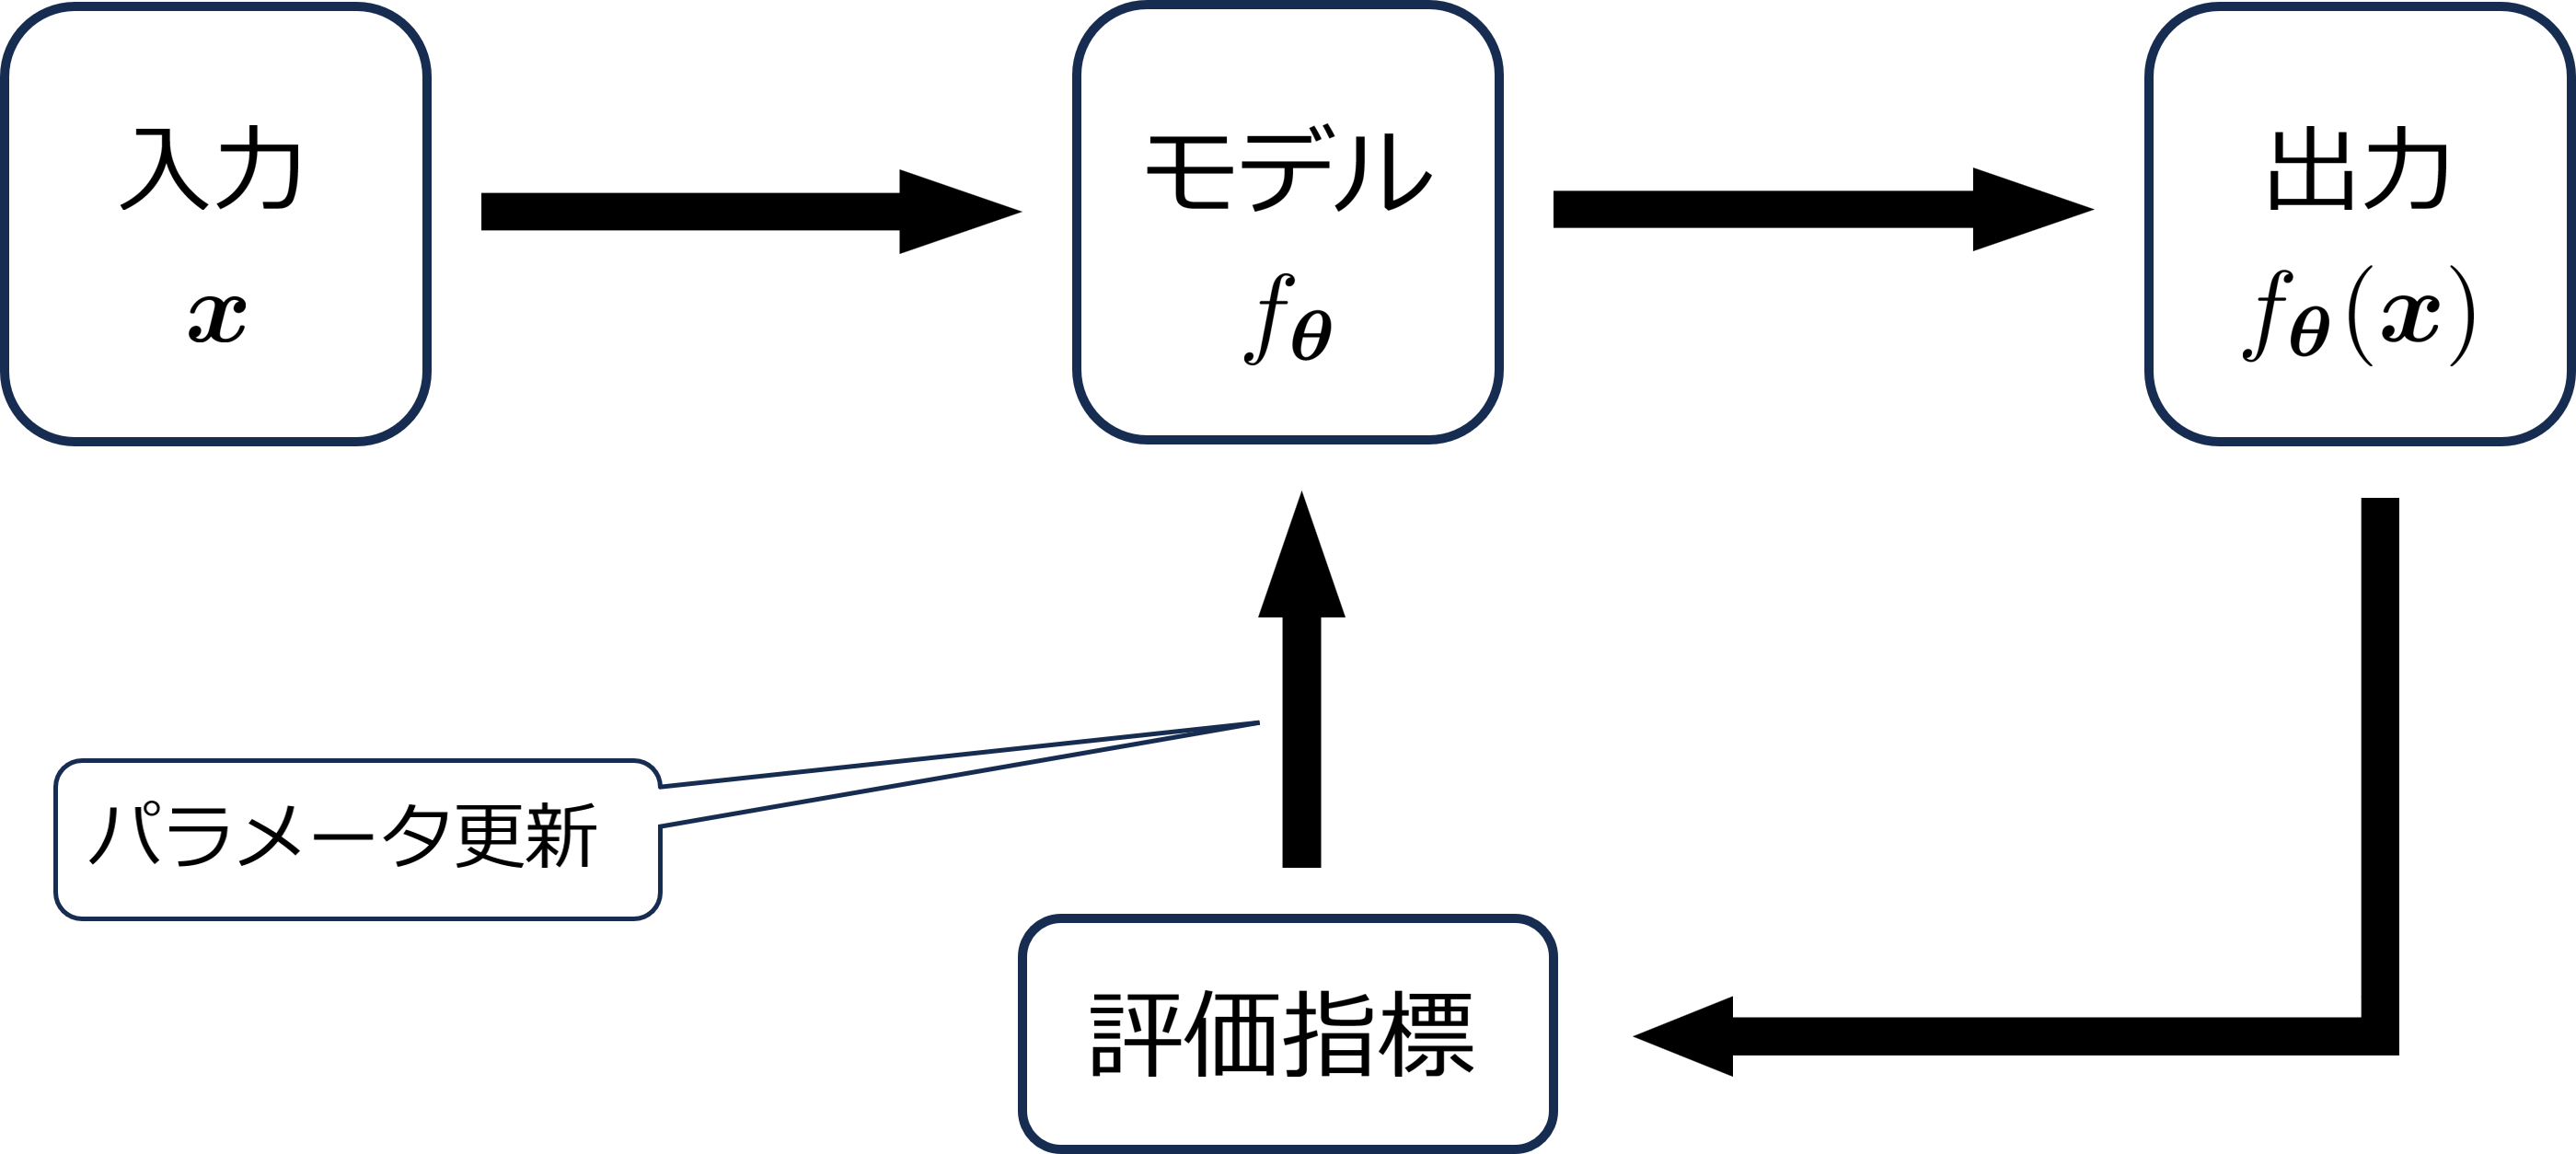
\includegraphics[height=6cm]{image/機械学習概要図.png}
    \caption{機械学習の大まかな流れ}
  \end{center}
\end{figure}
メトロポリス法とメトロポリス・ヘイスティング法は同じですか
\subsection{代表的なタスク}
ここでは,機械学習で解きたい問題であるタスクの代表的な例として「クラス分類」と「回帰」を紹介する.
\subsection*{クラス分類}
分類(classification)とは,データをいくつかのクラスに仕分ける作業のことである.例えば送られてきた電子メールをみて,それがスパムメールか通常メールを判別するような作業は,2クラス分類と呼べる.ここでのクラスというのは「スパムメールor通常メール」といった分類先のことを指す.ここで,スパムメールを$C_0$,通常メールを$C_1$とラベル付けしよう.また,入力データを$\bm{x}$とする.このとき,クラス分類というのは,与えられた$\bm{x}$が$C_0$と$C_1$のどちらに属するかを決定する作業である.数値的な変数$y = 0, 1$を導入すると,$\bm{x}$をクラス$C_{y}$へ分類するということは,$\bm{x}$の所属クラスを表す離散ベクトル$y(\bm{x})$の値を決めることであると言い換えられる.
\begin{equation}
  \bm{x} \longrightarrow y(\bm{x}) \in \{0, 1\}
\end{equation}
分類先のクラスが多数にわたる場合,多クラス分類とよび,分類先が$C_1,C_2,\dots,C_K$となり,ラベル$y(\bm{x})$も$1$から$K$の整数値をとる.これは先ほどの例でいえば,電子メールを「仕事」「家族」「友人」「スパム」と複数のファルダに分けることに対応する.
\subsection*{回帰}
データに対するクラス$y$は離散的とは限らない.例えば,過去数日の気象データ$\bm{x}$から明日の気温を予測したとき,$y$は温度の数値に相当し,連続的な実数値をもつ変数になる.このようにデータから,それに対応する実数値(を並べたベクトル)$\bm{y}$を予測作業のことを回帰(regression)という.つまり,回帰とは,与えられた$\bm{x}$を,対応する$\bm{y}$に変換するために関数$\bm{y}(\bm{x})$を決定する作業である.
\begin{equation}
  \bm{x} \longrightarrow \bm{y}(\bm{x}) \in \mathbb{R}
\end{equation}
\par
回帰による応用的なタスクとして,言語を翻訳する機械翻訳や音声を文字に起こす音声認識,状況が通常と異なることを自動的に検知させる異常検知,データのサイズを圧縮させるデータ次元削除などがあげられる.
\section{深層学習とは}
\section{統計入門}
機械学習とは,データ(経験)をもとにしてプログラムがいろいろなタスクをこなせるようにさせることであった.ではどのようにしたらプログラムはデータからタスクをこなすための知識を学びとれるか?データを科学的に分析する数理的手法といえば,統計学である.機械学習の手法もまた統計を基礎として構築される.そのような視点から特に統計的機械学習と呼ばれている.ここではまず,統計の基礎を確認し,どのようにして学習アルゴリズムや評価指標を設計できるかについて説明する.
\subsection{標本と推定}
まず,データ(集合)(data(set))やサンプル,標本(sample)という用語についてきちんと定めておく.これらはデータ点(data point)の集まりからなる.手書き文字による画像認識の例でいえば,データは統計分析に用いるために用意した画像の集合のことで,1枚1枚の画像がそれぞれデータ点とよばれる.ただしデータ点も略してデータとよばれる.さらにはサンプルをサンプルの要素であるデータ点の意味でも用いられる.これらは用語の乱用であり,全く正しくない用法であるが,しばしば用いられているのが現状であるため,本論文でも文脈に応じてこの使い方に準じることにする.\par
このようなデータ点(サンプル)の集まりからなるデータを分析するのが統計である.ここでは推定について考える.まず統計解析に用いるデータは,母集団から抽出(sampling)されたものとみなす.データの要素を1つ取り出すことは,正確には抜き取り(draw)という.そしてデータの分析から,データ自身ではなくその背後にある母集団についての知識を獲得することを目標とする.これは例えば疫学者が飲酒量と健康の関係を調べたいときに,地球上のすべての(=母集団)を調査する必要はないということと同じである.その代わりにランダムに選び取った(抽出した)少人数に対する調査結果(データ)を分析することで,人類すべてに通用する飲酒量と健康の相関関係を読み取ろうとするということである.\par
母集団の性質はデータ生成分布(generative distribution)$P_{\text{data}}(\mathrm{x})$により特徴づけられているものとする.つまり,不確実性を伴う現象を確率的にモデル化するということである.これは我々の手にするデータは,自然界におけるさまざまな物理的過程の結果,この宇宙に存在することになったわけだが,我々がその過程すべてやそこに寄与する因子のすべてを知ることはできないため,データを何らかの確率論的な過程に従ってランダムに生じているとみなしているということである.「サイコロを振ってどの目が出るか」という古典的な試行の例でも,もしサイコロやその周囲のすべての物理的情報を把握できるのであれば,原理的には出る目は力学で計算できるはずである.しかし人間には有限の認識・計算能力しかないため,どの目も1/6の確率で出るようにしか見えない.そこで今後はどの場合でも,$\bm{x}$という具体的なサンプルはデータ生成分布から抽出されたものであると仮定する.
\begin{equation}
  \bm{x} \sim P_{\text{data}}(\mathrm{x})
\end{equation}
このようにモデル化することでさまざまな現象を確率論的に予測することができる.ここで$x \sim P(\mathrm{x})$は,ある変数$\mathrm{x}$の実現値$x$が分布$P(\mathrm{x})$から生成している(生成された)ことを表す.\par
ここで抽出について1つ注意が必要である.我々は母集団について知りたいが,サンプルの抽出方法によって,結果に偏りが生じてしまっては困る.そこで基本的には無作為抽出されたデータのみを考えていくことにする.より正確には,すべてのサンプルは同一分布から独立に抽出されたものとする.\par
したがって母集団について知識を得るということは,データ生成分布を知ることを意味する.データを特徴づける十分な統計量をパラメータと呼ぶ.実際にはデータの生成の過程は極めて複雑なため,本当の$P(\mathrm{x})$は無数のパラメータをもっており,分布を完全に知ることはほぼ不可能である.そこで通常は$P(\mathrm{x})$をよく近似できると期待できるモデル分布$P(\mathrm{x};\bm{\theta})$を仮定し,そのモデルのパラメータ$\bm{\theta}$の最適値$\bm{\theta}^*$をデータから推定する.これはパラメトリックはアプローチと呼ばれる.パラメトリックなモデルを仮定したことで,分布を特徴付ける少数のパラメータの値を推定すればよいことになる.このようにデータ生成の過程について推論できれば,その結果を使うことで新規のデータに関してもいろいろと予測することができる.
\subsection{点推定}
データがある未知の分布から生成していると考え,この確率分布のパラメータを決定しようとするのが総計的推定である.我々は母集団に直接アクセスすることはできないため,手持ちの有限要素のデータ集合$\mathcal{D} = \{ x_1, x_2,\dots, x_N \}$からパラメータの尤もらしい値を計算するしかない.これを点推定という.点推定のため,データを決める確率変数$\{ \mathrm{x}_1, \mathrm{x}_2, \dots, \mathrm{x}_N \}$の関数である推定量
\begin{equation}
  \hat{\bm{\theta}}( \mathrm{x}_1, \mathrm{x}_2, \dots, \mathrm{x}_N )
\end{equation}
を作る.推定量のまた確率変数なので,データが具体的に与えられて,はじめて数値としてパラメータの推定値
\begin{equation}
  \hat{\bm{\theta}}^*( x_1, x_2, \dots, x_N )
  =\hat{\bm{\theta}}( x_1, x_2, \dots, x_N )
\end{equation}
を与えることになる.いずれにせよこの推定値は,いま考えているパラメータをよく近似するように作る.それによってデータの数値から,背後にある分布について知ることができる.\par
よい推定量の作り方にはいくつもの指標がある.そこで,ここでは推定量に推奨される性質をいくつか紹介する.

\subsubsection*{バイアスが小さい}
推定量のバイアスとは,推定量の期待値$\mathrm{E} \left[ \hat{\bm{\theta}} \right]$と真の値$\bm{\theta}^*$との差のことである.
\begin{equation}
  b\left( \hat{\bm{\theta}} \right)
  = \mathrm{E} \left[ \hat{\bm{\theta}} \right] - \bm{\theta}^*
\end{equation}
ここでの期待値は,データ生成分布での期待値なので,たくさんのデータ集合を用意して計算した平均値である.バイアスが小さいとは,推定量の偏りが小さく真の値から不要にズレていないということである.特にバイアスがゼロのものを不偏推定量と呼び,典型的な望ましい推定量である.一方でバイアスがあるものの,データの数が増えるにつれゼロへ漸近する状況$\lim_{N \rightarrow \infty} = 0$を漸近不偏推定量と呼ぶ.

\subsubsection*{分散が小さい}
分散は,真の値に対してどれだけ推定量がばらつくかを測っている.したがって,これが小さいことは望ましいのは明らかである.
\begin{equation}
  \text{Var}\left( \bm{\theta} \right)
  = \mathrm{E} \left[ \left( \hat{\bm{\theta}} - \bm{\theta} \right)^2 \right]
\end{equation}

\subsubsection*{一致性}
一致性とは,データ点の数を増えるにつれて統計量が真のパラメータに近づいていくという性質である.つまり,$N \rightarrow \infty$に従い
\begin{equation}
  \hat{\bm{\theta}}
  \rightarrow \bm{\theta}^*
\end{equation}
となるということである.この性質を満たす推定量を一致推定量と呼ぶ.

\subsubsection{ガウス分布の場合}
ガウス分布とは実数値をとる確率変数$x$上の次のような分布である.
\begin{equation}
  P(x)
  = \mathcal{N}(x; \mu, \sigma^2)
  = \frac{1}{\sqrt{2 \pi \sigma^2}} e^{-\frac{(x-\mu)^2}{2\sigma^2}}
\end{equation}
$\mu$と$\sigma^2$の2つを決めればこの分布が定まるため,この2つがパラメータである.では,ガウス分布から無作為に取り出した$N$個のデータからパラメータを推定するにはそうすればよいか.今,どのサンプルも無作為に抽出されているとしたため,任意のデータ点$\mathrm{x}_n$はガウス分布に従う独立な確率変数である.したがって,その期待値は分布のパラメータ$\mu$に一致している.
\begin{equation}
  E_{\mathcal{N}}[\mathrm{x}_n]
  = \int_{-\infty}^{\infty} x_n P(x_n) dx_n
  = \mu
\end{equation}
これはもちろん分布に対する期待値だが,それを与えられたデータ$\mathcal{D} = \{ x_1, x_2, \dots, x_N \}$に関する平均値で近似してみる.つまり,本当の期待値であるガウス分布の期待値をサンプル平均で置き換えたものを$\mu$の推定量$\hat{\mu}$とするのである.
\begin{equation}
  \hat{\mu}
  = \frac{1}{N} \sum_{n=1}^{N} \mathrm{x}_n
\end{equation}
すると,これは見事に不偏推定量になっている.
\begin{align}
  E_{\mathcal{N}}[\hat{\mu}]
   & = \frac{1}{N} \sum_{i=1}^N \mathrm{E}[\mathrm{x}_n] \notag \\
   & = \mu
\end{align}
では,$\sigma^2$はどうなっているか.
\begin{align}
  \mathrm{E}_{\mathcal{N}}[(\mathcal{X}_n - \mu)^2]
   & = \int_{-\infty}^{\infty} (x_n - \mu)^2 P(x_n) dx_n \notag \\
   & = \sigma^2
\end{align}
となる.したがって安直には,再びこの期待値をサンプル平均で近似すれば推定量$\hat{\sigma}^2$が得られると思う.
\begin{equation}
  \hat{\sigma}^2
  = \frac{1}{N} \sum_{n=1}^N (x_n - \hat{\mu})^2
\end{equation}
これが不偏であるか見るために期待値を計算する.
\begin{align}
  \mathrm{E}_{\mathcal{N}}[(\mathrm{x}_n - \hat{\mu})^2]
   & = \mathrm{E}_{\mathcal{N}}[(\mathrm{x}_n - \mu)^2 -2(\mathrm{x}_n - \mu)^2 - 2(\mathrm{x}_n - \mu)(\hat{\mu} - \mu) + (\hat{\mu} - \mu)^2] \notag \\
   & = \sigma^2 -2 \frac{\sigma^2}{N} + \frac{\sigma^2}{N}
\end{align}

\begin{align*}
  \mathrm{E}_\mathcal{N}\left[\hat{\sigma}^2\right]
   & =\mathrm{E}_\mathcal{N}\left[\frac{1}{N} \sum_{n=1}^N\left(\mathrm{x}_n-\hat{\mu}\right)^2\right]                                                                                                                                       \\
   & =\frac{1}{N} \mathrm{E}_\mathcal{N}\left[\sum_{n=1}^N\left\{\left(\mathrm{x}_n-\mu\right)^2-2\left(\mathrm{x}_n-\mu\right)(\hat{\mu}-\mu)+(\hat{\mu}-\mu)^2\right\}\right]                                                                       \\
   & =\frac{1}{N}\left\{\sum_{n=1}^N \mathrm{E}_\mathcal{N}\left[\left(\mathrm{x}_n-\mu\right)^2\right]-2 \sum_{n=1}^N \mathrm{E}_N\left[\left(\mathrm{x}_n-\mu\right)(\hat{\mu}-\mu)\right]+N \mathrm{E}_N\left[(\hat{\mu}-\mu)^2\right]\right\}                       \\
   & =\sigma^2-\frac{2}{N^2} \sum_{n=1}^N \sum_{m=1}^N \mathrm{E}_\mathcal{N}\left[\left(\mathrm{x}_n-\mu\right)\left(\mathrm{x}_m-\mu\right)\right]+\frac{1}{N^2} \sum_{n=1}^N \sum_{m=1}^N \mathrm{E}_\mathcal{N}\left[\left(\mathrm{x}_n-\mu\right)\left(\mathrm{x}_m-\mu\right)\right] \\
   & =\sigma^2-\frac{1}{N^2} \sum_{n=1}^N \mathrm{E}_\mathcal{N}\left[\left(\mathrm{x}_n-\mu\right)^2\right]                                                                                                                                 \\
   & =\sigma^2-\frac{1}{N} \sigma^2                                                                                                                                                                              \\
   & =\left(1-\frac{1}{N}\right) \sigma^2
\end{align*}
となり,不偏ではない.ただし,$N \rightarrow \infty$の極限でこの期待値は$\sigma^2$に一致するため,漸近的不偏推定量になっている.また,バイアスのない推定量は余分な係数を除いたものなので,
\begin{equation}
  \hat{\tilde{\sigma}}^2 
  = \frac{1}{N - 1} \hat{\sigma^2} = \frac{1}{N - 1} \sum_{n=1}^N (\mathrm{x}_n - \hat{\mu})^2
\end{equation}
と与えられる.

\subsubsection{ベルヌーイ分布の場合}
コイン投げの結果が表裏どちらかなど,2つのランダムな値をとる現象を記述するのがベルヌーイ分布である.確率変数を0か1の離散値をとるものとし,$\mathrm{x}$が1をとる確率を$p$とすると,この分布は,
\begin{equation}
  P(x) = p^x (1 - p)^{1-x}
\end{equation}
と書ける.パラメータは$p$のみである.ベルヌーイ分布の期待値と分散は,
\begin{equation}
  \mathrm{E}_{P}[\mathrm{x}] 
  = \sum_{\mathrm{x} = 0,1} x P(x) 
  = 1 \cdot P(1) 
  = p
\end{equation}
\begin{align}
  \mathrm{E}_{P}[(\mathrm{x} - p)^2] 
  &= \sum_{\mathrm{x} = 0,1} (x -2px + p^2) P(x) \notag \\
  &= p^2 \cdots P(0) + (1 - 2p + p^2) \cdot P(1) \notag \\
  &= p(1-p)
\end{align}
と書くことができる.すると,パラメータの推定量は再びサンプル平均
\begin{equation}
  \hat{p} 
  = \frac{1}{N} \sum_{n=1}^N x_n
\end{equation}
がよさそうである.実際,
\begin{equation*}
  \mathrm{E}_{P}[\hat{p}] = \frac{1}{N} \sum_{N=1}^{n} E_P[\mathrm{x}_n]  
\end{equation*}
であり,データサイズが大きくなるほど推定値のばらつきがゼロに近づいていく,したがって大きなデータに対して分散は小さくなるような推定量である.

\subsection{最尤推定}
これまで,発見的な方法で推定量を探してきたが,これでは複雑な分布の場合はどうしようもない.ところがパラメトリックな場合には,実は広く使える強力な手法がある.これが最尤推定法である.\par
データ生成分布のパラメトリックモデル$P_{\text{model}}(\mathrm{x}; \bm{\theta})$が与えられているとする.与えられたサンプル$\mathcal{D} = \{x_1, x_2, \dots, x_N\}$は,この分布から無作為に抽出されていると近似する.すると,これらは独立に同じモデルから生成された実現値なので,このデータ集合が得られる同時確率は
\begin{equation*}
  P(x_1, x_2, \dots, x_N; \bm{\theta}) 
  = \prod_{n=1}^N P_{\text{model}}(x_n; \bm{\theta})
\end{equation*}
である.これを変数$\bm{\theta}$に対する量とみなして$L(\bm{\theta}) = P(x_1, x_2, \dots, x_N; \bm{\theta})$と書き,尤度関数と呼ぶ.データ値が$\{ x_1, x_2, \dots, x_N \}$という観測値を取ったのは,パラメータ$\bm{\theta}$の値が確率$P(x_1, x_2, \dots, x_N; \bm{\theta})$を大きくするようなものであったからであると考える.つまり,$L(\bm{\theta})$を最大にするようなパラメータ値であるためにデータ$\{ x_1, x_2, \dots, x_N \}$が実現されやすかったと解釈するのである.すると,与えられたデータに対して尤もらしいパラメータの値は尤度を最大化したものということになる.
\begin{equation}
  \bm{\theta}_{ML} = \underset{\bm{\theta}} {\operatorname{argman}} L(\bm{\theta})
\end{equation}
ただし,尤度は確率の積であるため,1以下の数値を何回も掛け合わせた値になる.値が小さすぎると計算機上でアンダーフローを起こしうるため,実用上,対数尤度関数を最大化する.\par
\begin{equation}
  \bm{\theta}_{ML} = \underset{\bm{\theta}} {\operatorname{argman}} \ln{L(\bm{\theta})}
\end{equation}
このように何らかの目的関数を最大化,あるいは最小化することで推定に用いる最適なパラメータ値を決定するのが機械学習における常套手段である.実際,多くの機械学習アルゴリズムは最尤法を基礎に構築される.機械学習では,最大値よりも最小値をして問題を書くことが多いので,負の対数尤度を目的関数とした最小化問題として表現する.
\begin{equation}
  \bm{\theta}_{ML} = \underset{\bm{\theta}} {\operatorname{argmin}} (-\ln{L(\bm{\theta})})
\end{equation}

\subsubsection{ガウス分布の場合}
ガウス分布の例を考える.$N$個のデータに対する尤度関数は
\begin{equation}
  L(\bm{\theta})
  = \prod_{n=1}^N \frac{1}{\sqrt{2 \pi \sigma^2}} e^{-\frac{(x_n - \mu)^2}{2 \sigma^2}}
\end{equation}
である.ただし,$\bm{\theta} = (\mu, \sigma^2)$として2つのパラメータをまとめて表記した.対数尤度関数はもう少しシンプルで
\begin{equation}
  \ln{L(\bm{\theta})}
  = -\frac{N}{2} \ln{\sigma^2} - \sum_{n} (x_n - \mu)^2 + \text{const.}
\end{equation}
となる.この関数の最大値を探すには,微分係数がゼロの場所を求めればよいので,
\begin{align}
& \left.\frac{\partial \ln L(\bm{\theta})}{\partial \mu}\right|_{M L}
= \frac{1}{\sigma_{M L}^2} \sum_{n=1}^N\left(x_n-\mu_{m L}\right) = 0 \\
& \left.\frac{\partial \ln L(\bm{\theta})}{\partial \sigma^2}\right|_{\mu L}
= -\frac{N}{2 \sigma_{M L}^2}+\frac{1}{2\left(\sigma_{M L}^2\right)^2} \sum_{n=1}^N\left(x_n-\mu_{M L}\right)^2 = 0
\end{align}
を解けばよい.これはすぐに解け,得られる推定量$(\mu_{ML}, \sigma_{ML}^2)$は先ほど見つけた推定量$(\hat{\mu}, \hat{\sigma^2})$と一致する.

\subsubsection{ベルヌーイ分布の場合}
ベルヌーイ分布に対しては,対数尤度は
\begin{equation}
  L(p) = \prod_{n=1}^{N} p^{x_n} (1 - p)^{1 - x_n}
\end{equation}
となる.よって対数尤度は
\begin{equation}
  \ln{L(p)} = \sum_{n=1}^{N} (x_n \ln{p} + (1 - x_n)\ln{(1 - p)})
\end{equation}
となる.これを解いて得られる最尤推定量$p_{ML}$もまた,先ほど求めた推定量と一致している.このように最尤法は推定量を求めるための汎用性のある方法である.

\section{機械学習の基礎}
機械学習ではデータ集合を学習アルゴリズムで処理することでコンピュータプログラムを学習させる.それによって,プログラムが与えられたタスクをよりうまくこなせるようにすることを目標にする.データ(集合)は機械学習の文脈では訓練データと呼ばれる.\par
学習を担うのは,人間がデザインする学習機械(アーキテクチャ)である.アーキテクチャの学習プロセスを決めているのが学習アルゴリズムで,これもまた人間が設計する.アルゴリズムの詳細は学習させたいタスクやデータの種類によって変わる.ただし,一般的な設計思想は,まず与えられたタスクに対するパフォーマンスの良さを測る尺度を導入し,その値を改善するようなアルゴリズムを実現するというものである.この評価尺度を損失関数や誤差関数と呼ぶ.

\subsection{教師あり学習}
機械学習には教師あり学習や教師なし学習,強化学習など,いくつもの枠組が知られているが,深層学習の基礎になるものは教師あり学習である.教師あり学習の特徴は,用意すべき訓練データが必ず入力$\bm{x}$と出力$\bm{y}$のペアの形をとることである.つまり,訓練データは$\mathcal{D} = \{ (\bm{x_1}, \bm{y_1}), \dots, (\bm{x_N}, \bm{y_N}) \}$という形をしている.機械学習の目的はこの入出力間の関係を推定することで,新しい未知の$\bm{x}$が与えられたときに対応する出力$\bm{y}$を適切に予測できるようになることである.\par
\begin{equation}
  \bm{x} \longrightarrow \bm{y}
\end{equation}
統計学的な用語でいえば,説明変数$\mathrm{x}$と目標変数$\mathrm{y}$の間の関係式を知り,常に目標変数を予測できるモデルを作ろうということである.そのために目標変数の適切な推定量$\hat{y}$を探すのが学習である.実際には推定量の関数モデルを仮定して,そのパラメータを訓練データから最適化する学習アルゴリズムを実装する.

\subsection{最小二乗法による線形回帰}
入力$\bm{x}$から出力$y$を予測するのが回帰であった.ここでは出力がベクトルではなくスカラーの場合を考える.そして,ここではパラメトリックなモデルを考える.つまり,常に$y$はある関数$\hat{y} = f(\bm{x}; \bm{w})$で表される規則で$\bm{x}$が決まっているとする.ただし,この関数のパラメータ$\bm{w}$はまだ未知であり,与えられたデータから最適なパラメータ値を決める作業が学習に相当する.また,データの観測には常にランダムなプロセスに起因する不確実な要素が介在するため,その効果をノイズ$\epsilon$として,
\begin{equation}
  y = f(\bm{x}; \bm{w}) + \epsilon
\end{equation}
のようにモデル化する.ここで$\epsilon$は確率変数で,ランダムなノイズによる規則性のかき乱しを表す.その一方で我々が知りたいのは$\bm{x}$と$y$の間の対応規則を捉える項$f(\bm{x}; \bm{w})$である.\par
ここで考えるのは,特に規則性の部分がパラメータの1次関数であることを仮定した回帰モデルである.
\begin{equation}
  f(\bm{x}; \bm{w})
  = \bm{w}^{\top} \bm{h}(x) 
  = \sum_{j=0} w_j h_j(\bm{x})
\end{equation}
これはパラメータに対して線形であるため線形回帰と呼ばれる.一方で$h_j(\bm{x})$は必ずしも線形関数である必要はない.例えば,入力$x$がベクトルではなくスカラーの場合,$h_j(x) = x^j$という単項式を選んだ場合がいわゆる多項式回帰である.
\begin{equation}
  f(x; \bm{w}) = \bm{w}^{\top} \bm{h}(x) = \sum_{j=0}^M w_j x^j
\end{equation}
この多項式回帰も線形回帰の一種であることに注意.\par
回帰分析ではモデル$f(\bm{x}; \bm{w})$が与えられたデータ$\mathcal{D}$の入出力が満たす対応関係によく当てはまるように,モデルのパラメータ$\bm{w}$を調整する.そのためにはモデルがどの程度データに当てはまっているかを測る尺度が必要である.機械学習では特に,モデル$f(\bm{x}; \bm{w})$をパフォーマンスの悪さを測る尺度である誤差関数を最小化することにより最適パラメータ$\bm{w}^*$を決定する.最も有名で理解しやすい誤差関数として,平均二乗誤差がある.
\begin{equation}
  E_{\mathcal{D}}(\bm{w})
  = \frac{1}{N} \sum_{n=1}^{N}(\hat{y}(\bm{x}_n; \bm{w}) - y_n)^2
\end{equation}
$\hat{y}(\bm{x}_n; \bm{w})$はモデルに$n$番目の入力データを入れて得られるモデル予測であり,$y_n$が実際にデータに対応した出力値である.したがって,$(\hat{y}(\bm{x}_n; \bm{w}) - y_n)^2$は予測と正解の差を2乗したものである.これはまさに予測と正解のズレを測っており,それを全サンプルについて平均したものがこの誤差関数である.平均二乗誤差を最小化するこの方法が,平均二乗法である.\par
探したいモデルは,できるだけデータへ当てはまりがよいものであるため,この誤差関数を最小化するようなパラメータ値
\begin{equation}
  \bm{w}^* = \underset{\bm{\theta}} {\operatorname{argmin}} (E_{\mathcal{D}}(\bm{w}))
\end{equation}
を$\hat{y}$のパラメータ値に選んだものが探していたモデルということになる.\par
ここで1つ概念的な注意を述べておく.機械学習の本来の目的は,手持ちの訓練データだけでなく,ありとあらゆるデータに対してよい性能を示すモデルを作ることである.訓練データをもとにして学習機械を訓練し,未知のデータに対してまでよく働く状況が実現されることを汎化という.したがって汎化を達成するために本来最小化すべき誤差関数は汎化誤差ということになる.
\begin{equation}
  E_{\text{gen}}(\bm{w}) 
  = \mathrm{E}_{(\mathbf{x}, \mathrm{y}) \sim P_{\text{data}}} \left[ (\hat{\mathrm{y}}(\mathbf{x}; \bm{w}) - y)^2 \right]
\end{equation}
しかしながら,有限な能力しかない我々には,可能なすべてのデータを集めてくることはできない.したがって,この「本物」誤差を最小化することは不可能である.そこで機械学習では手持ちのデータのサンプル平均で汎化誤差を近似的に見積もり,それを最小化している.式(\ref{})のようなサンプル平均で作った誤差を訓練誤差という.訓練誤差を小さくしただけでは,汎化がそう易々と実現するとはなかなか言えない.しかし驚くべきことに,訓練誤差の最小化によって汎化に近づくことができる.

\subsection{過適合と汎化}
ここでは,汎化の実現がそう簡単ではないことを説明する.\par
簡単のために1次元データの多項式回帰を考える.つまり,与えられた入力$x$から出力$y$を予測する規則性を推定するために,多項式モデル
\begin{equation}
  \hat{y} = \sum_{j=0}^M w_j x^j
\end{equation}
をデータにフィッティングする.この際,多項式の次数$M$は我々が選ばなくてはならない.このようにモデルの選択時に決めなければならないパラメータをハイパーパラメータと呼び,学習されるパラメータを区別する.ハイパーパラメータ自体は学習アルゴリズムでは一切修正されない.この場合,$M$の重みパラメータの個数も決定しているため,まさにモデルの自由度を与えている.図\ref{線形回帰}はフィッティングの結果である.$M=1$に対応する図\ref{線形回帰}(a)のように,データの豊かさに対してモデルの自由度が小さすぎると,データの構造を捉えることはまったくできない.つまり,訓練誤差の値が大きすぎて,これでは何の予測能力の得られないだろう.このような状況はアンダーフィッティングと呼ばれる.\par
そこで$M$をどんどん大きくしていくことで,データの複雑な構造をよりよく捉えられるようになるのではないかと考えられる.しかし,不必要に大きな自由度をもったモデルは,異なる問題を引き起こす.というのも,モデルの自由度が大きすぎると,学習データのもつノイズ(統計的なゆらぎ)までをも多項式モデルが正確にフィッティングしてしまうのである.これが図\ref{線形回帰}(c)の状況である.すると,与えられた訓練データに関する誤差関数に値は確かにどんどん小さくできるが,未知のデータに対してはどんどん予測能力を失っていく.この状況は過学習と呼ばれる.\par
このようにモデルの自由度を減らしていくと過学習は下げられるがどんどん訓練誤差が大きくなり,逆に自由度を大きくしていくと訓練誤差をいくらでも小さくできる一方で過学習が起こって汎化誤差が増え始めてしまうトレードオフの状況になっている.すると,我々が見つけたい汎化の状況は2状態の中間である図(\ref{})(b)にあると考えられる.これはモデルの自由度と学習すべきデータを含む情報の豊かさがつり合う状況である.したがって機械学習をうまくいかせるためには,まずちょうどよいモデルパラメータの数,つまりモデルの自由度を見積もらなくてはならない.自由度の見積もりにはいろいろな基準があるが,残念なことに深層学習のような複雑なモデルではどれもあまり役立たないのが現状である.そこで実務の場面では,学習に用いるデータとは別に検証用のデータを用意して
検証用データに関する誤差を目安に,仮定したモデルがよいものかどうかを見極めることになる.
\begin{figure}[htbp]
  \begin{minipage}[b]{0.3\linewidth}
    \centering
    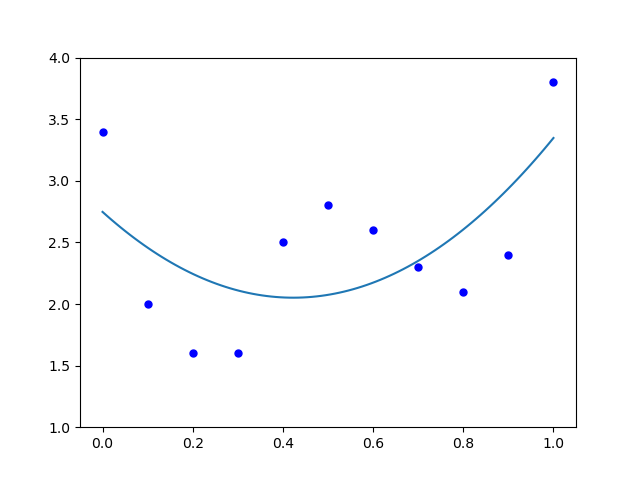
\includegraphics[keepaspectratio, scale=0.3]{image/多項式回帰(a).png}
    \subcaption{アンダーフィッティング}
  \end{minipage}
  \begin{minipage}[b]{0.3\linewidth}
    \centering
    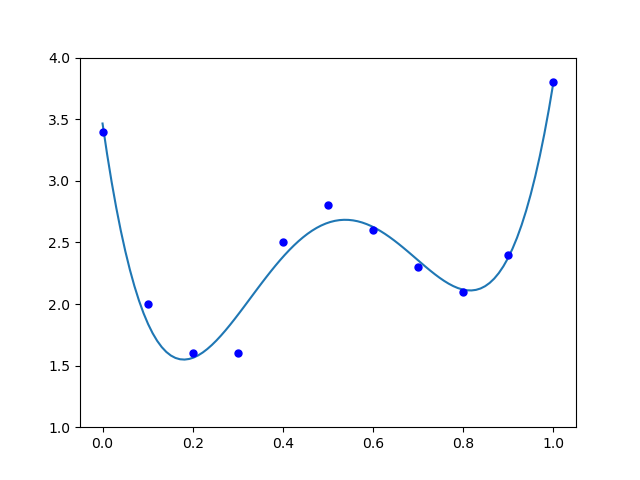
\includegraphics[keepaspectratio, scale=0.3]{image/多項式回帰(b).png}
    \subcaption{適切なパラメータ数}
  \end{minipage}
  \begin{minipage}[b]{0.3\linewidth}
    \centering
    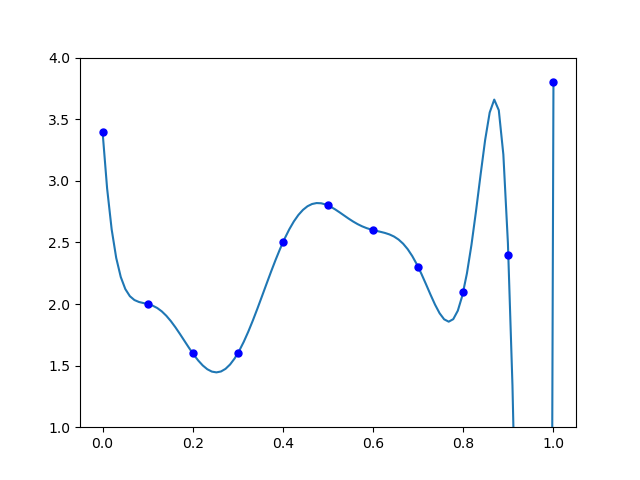
\includegraphics[keepaspectratio, scale=0.3]{image/多項式回帰(c).png}
    \subcaption{過学習}
  \end{minipage}
  \caption{1次元データの線形回帰の例}
  \label{線形回帰}
\end{figure}

\subsection{正則化}
過学習を避けるための一番わかりやすい方法は,自由度の数が大きすぎないモデルをはじめから選んでおくことである.自由度を実質的に減らしてしまうさまざまな手法は正則化と呼ばれる.実はモデル自体を修正することなく,学習アルゴリズムを少し変更するだけで実質的な自由度を減らすことができる.一般的にこのような正則化は,最適化すべき誤差関数の変更として表現することができる.
\begin{equation}
  E_{\text{new}}(\bm{w}) 
  = E(\bm{w}) + \lambda R(\bm{w})
\end{equation}
$\lambda$は正則化の効果の大きさを調整するための正則化パラメータである.\par
重み減衰(weight decay)はこのような正則化の代表例である.多項式回帰の例からわかるように,もし強制的に多くのパラメータの値を0に制限することができれば,はじめから調整できるパラメータが少ないため自由度を減らしたことと同じことになる.そこで最小化する誤差関数に,次のような項を加えてみる.
\begin{equation}
  E_{\text{wd}}(\bm{w}) 
  = E(\bm{w}) + \lambda \bm{w}^{\top} \bm{w}
\end{equation}
新たに項に加わった右辺全体を最小化するということは,重みベクトルのノルム$\bm{w}^{\top} \bm{w}$をできる限り小さくする解$\bm{w}^*$がより好まれるようになるということである.そのため,このように修正された後の最適解では,可能な限りの$\bm{w}$の成分がほぼゼロになっている.したがって重み減衰はモデル自体を変えずに,最小化する誤差関数へのパラメータ数を減らすペナルティ項を加える正則化である.回帰に重み減衰を適用したものはRidge回帰と呼ばれる.\par
Ridge回帰以外にも,さまざまな回帰の正則化が存在する.その一例は
\begin{equation}
  E_{\text{wd}}(\bm{w}) 
  = E(\bm{w}) + \lambda \sum_i |w_i|
\end{equation}
という誤差関数と用いるLASSO回帰である.この手法もまた,不要な重みをできるだけゼロへ近づける効果がある.\par
与えられたタスクのパフォーマンス向上という目標は維持しつつも,モデルの自由度を減らして過学習を避ける正則化の手法は,汎化性能の実現を目指す機械学習では極めて重要な位置を占める.


\subsection{クラス分類}
クラス分類の教師あり学習について説明する.クラス分類とは与えられた入力$\bm{x}$を$K$個のクラス$\mathcal{C}_1, \mathcal{C}_2, \dots, \mathcal{C}_K$へ分類する作業である.これらのクラスは互いに排他的であり,1つの入力が複数のクラスにまたがって所属することはないとする.また,入力には,必ず1つの所属先があるものとする.回帰のように数値的に扱うために,離散的な目標変数を導入する.
\subsubsection*{2値分類の場合}
分類先が2つしかない状況では,1つ目のクラスに属していることを$y=1$,2つ目のクラスに属していることを$y=0$として表現する2値変$y$を用いればよい.
\subsubsection*{多クラス分類の場合}
手書き数字$0 \sim 9$のどれかを判定する場合など,分類先クラスが複数ある場合はいろいろなアプローチがある.最もシンプルなものは,$K$個のクラスそれぞれに対応して$y = 1, 2, \dots, K$という$K$個の値をとる離散変数を用いる方法である.手書き数字の例では$K = 10$である.この変数を,ベクトルを用いた別の表現である,1-of-hot符号化に写像できる.$y$によって決まる$K$成分ベクトル
\begin{equation}
  bm{t}(y) = \begin{pmatrix}
    t(y)_1 & t(y)_2 & \cdots & t(y)_K
  \end{pmatrix}^{\top}
\end{equation}
が1-of-hot符号化である.この手法では入力が$k$番目のクラスに属している.つまり,$y=k$であることを,第$k$成分が$t(y=k)_{k} = 1$でそれ以外の成分$t(y=k)_{l \neq k}$はすべて0であることで表現している.このような表現法をone-hot表現と呼ぶ.例えば一番のクラスに属しているのであれば,
\begin{equation}
  \bm{t}(y=1) = \begin{pmatrix}
    1 & 0 & \cdots & 0
  \end{pmatrix}^{\top}
\end{equation}
ということである.ここで,クロネッカーのデルタ記号
\begin{equation}
  \delta_{i, j} 
  = \begin{cases}
    1 & (i = j) \\
    0 & (i \neq j)
  \end{cases}
\end{equation}
を使うと,one-hot表現ベクトルの成分は
\begin{equation}
  t(y)_k = \delta_{y, k}
\end{equation}
と書くことができる.

\subsection{クラス分類へのアプローチ}
クラス分類では与えられた入力に対し,離散的な目標変数を予測したいわけだが,そのためには複数のアプローチが考えられる.

\subsubsection*{関数モデル}
関数モデルは,入力と出力の間の関係を関数としてモデル化する方法である.
\begin{equation}
  \hat{y} = y(\bm{x}; \bm{w})
\end{equation}
例えば0,1の2値をとる目標変数に対し,
\begin{equation}
  y(\bm{x}; \bm{w}) = f(\bm{w}^{\top} \bm{x} + b)
\end{equation}
というモデルを仮定すると,これは1層ニューラルネットワークになっている.

\subsubsection*{生成モデル}
関数モデルによるアプローチ以外の手法では,データを確率的に取り扱う.生成モデルではデータに潜むランダム性を同時分布$P(\bm{x}, \bm{y})$のモデル化により表現し,このモデルをデータにフィットさせる.$k$成分だけが1の$\bm{t}(\bm{y})^{\top} = \begin{pmatrix} 0 & \cdots & 0 & 1 & 0 & \cdots & 0 \end{pmatrix}$に対する$P(\bm{x}, \bm{y})$は,入力が$\bm{x}$で所属クラスが$\mathcal{C}_k$である確率を意味する.この代わりに$P(\bm{x}, \mathcal{C}_k)$をモデル化しても同じことである.\par
この確率をすべてのクラスについて求めたあと,$\bm{x}$について周辺化して$P(\bm{x})$を求めてベイズの公式を使うことで条件付き確率$P(\mathcal{C}_k | \bm{x})$を求める.$P(\mathcal{C}_k | \bm{x})$がわかれば任意のデータ$\bm{x}$がわかれば任意のデータ$\bm{x}$が各クラスに属している確率が評価でき,得られた確率の値がもっとも大きくなるクラス$\mathcal{C}_k$を$\bm{x}$の所属先と予測することになる.

\subsubsection*{識別モデル}
生成モデルではまず同時分布を得て,そこから条件付き確率分布$P(\mathcal{C}_k | \bm{x})$を計算していた.このような回りくどいことをせずに$P(\mathcal{C}_k | \bm{x})$おモデル化してデータに学習させるのが認識モデルである.予測する方法は生成モデルと同様である.

\subsection{ロジスティック回帰}
クラス分類を例にとって,識別モデルをもう少し詳しく見ていく.まずは2クラス分類から考える.この場合はクラスが2つしかないため,確率分布は$P(\mathcal{C} | \bm{x}) = P(\bm{x} | \mathcal{C}) = 1$を満たす.ここでシグモイド関数
\begin{equation}
  \sigma(u) 
  = \frac{1}{1 + e^{-u}}
  = \frac{e^u}{1 + e^u}
\end{equation}
を導入する.今考えていた,条件付き確率は
\begin{equation}
  P(\mathcal{C}_1 | \bm{x})
\end{equation}
とシグモイド関数で書くことができる.ここで,$u$は対数オッズと呼ばれる因子で
\begin{equation}
  u 
  = \ln{\frac{P(\mathcal{C}_1 | \bm{x})}{1 - P(\mathcal{C}_1 | \bm{x})}}
  = \ln{\frac{P(\mathcal{C}_1 | \bm{x})}{P(\mathcal{C}_2 | \bm{x})}}
\end{equation}
である.
\begin{equation}
  e^u
  = \frac{P(\mathcal{C}_1 | \bm{x})}{P(\mathcal{C}_2 | \bm{x})}
\end{equation}
がオッズ比と呼ばれ,$\mathcal{C}_1$である確率とそうでない確率の比率を表す.対数オッズが0を超えると$\mathcal{C}_1$である確率が$\mathcal{C}_2$である確率を上回ることになる.したがって対数オッズも明快な意味をもつため,確率モデルを設計する際に基本的な道具となる.\par
実際多くのクラス分類では,対数オッズ$u$が入力に関する線形関数であることを仮定した単純な確率モデルが用いられる.
\begin{equation}
  u = \bm{w}^{\top} \bm{x} + b
\end{equation}
$\bm{w}$はモデルのパラメータをまとめて表したベクトルである.このモデルは統計分析においてロジスティック回帰と呼ばれ,ベルヌーイ分布の統計分析法として広く用いられている.また,ロジスティック回帰は,一般化線形モデルという重要な統計モデルの典型例である.\par
訓練データとのフィッティングには最尤法を用いる.これもまた,一般化線形モデル全般に通じる方法である.まず離散数値をとる目標変数$y$は,$y=1$が1つ目のクラス$\mathcal{C}_1$に入っている場合,$y=0$が$\mathcal{C}_2$に入っている場合を表していた.つまり,
\begin{equation}
  P(y=1 | \bm{x})
  = P(\mathcal{C}_1 | \bm{x}), \quad
  P(y=0 | \bm{x})
  = 1 - P(\mathcal{C}_1 | \bm{x}), \quad
\end{equation}
である.$P(y | \bm{x})$はベルヌーイ分布なので,一般的に次のように書ける.
\begin{equation}
  P(y|\bm{x})
  = \left( P(\mathcal{C}_1)|\bm{x} \right)^y \left( 1 - P(\mathcal{C}_1)|\bm{x} \right)^{1 - y}
\end{equation}
これは右辺に$y = 1$と$y = 0$を実際に代入すればすぐに理解できる.したがって,これをデータ$\{ (\bm{x}_1, y_1), \cdots, (\bm{x}_N, y_N) \}$によって学習させるには,最尤法に従って,次の尤度関数
\begin{equation}
  L(\bm{w}) 
  = \prod_{n=1}^N \left( P(\mathcal{C}_1)|\bm{x}_n \right)^{y_n} \left( 1 - P(\mathcal{C}_1)|\bm{x}_n \right)^{1 - y_n}
\end{equation}
を最大化すればよかった.ここでロジスティック回帰のパラメータ$\bm{w}$は,対数オッズの部分を線形関数でモデル化した際に式(\ref{})で挿入されたパラメータであったことを思い出しておこう.機械学習の実装で用いられるのは対数尤度であったので,負の対数尤度で誤差関数を定義する.
\begin{equation}
  E(\bm{w}) 
  = -\sum_{n=1}^{N} \left( y_n \ln{P(\mathcal{C}_1|\bm{x}_n)} + (1 - y_n)\ln{(1 - P(\mathcal{C}_1|\bm{x}_n))} \right)
\end{equation}
これはデータの経験分布とモデル分布の間の交差エントロピーと呼ばれ,深層学習でもよく登場する重要な誤差関数の1つである.

\subsection{ソフトマックス回帰}
多クラス分類の識別モデルについて考える.この場合もロジスティック回帰の一般化で取り扱うことができる.次の式に注目する.
\begin{equation}
  P(y | \bm{x}) 
  = \prod_{k=1}^{K} (P(\mathcal{C}_k | \bm{x}))^{t(y)_k}
\end{equation}
これが正しい式であることは,one-hot表現の定義である式(\ref{})からわかる.例えば,これは$\bm{t}(y) = \begin{pmatrix} 1 & 0 & 0 & \dots \end{pmatrix}^{\top}$に対応した$y$を考えたならば,式(\ref{})の右辺は$P(\mathcal{C} | \bm{x})$となるからである.この分布はベルヌーイ分布の多値変数への自然な拡張である,マルチヌーイ分布やカテゴリカル分布と呼ばれる.この分布を少し書き換えてみると,$\sum_{k=1}^{K} t(y)_k = 1$が常に成り立っているため,
\begin{align}
  P(y | \bm{x}) 
  &= \prod_{k=1}^{K-1} (P(\mathcal{C}_k | \bm{x}))^{t(y)_k} (P(\mathcal{C}_K | \bm{x}))^{1 - \sum_{k=1}^{K-1} t(y)_k} \notag \\
  &= (P(\mathcal{C}_K | \bm{x})) \prod_{k=1}^{K-1} \left( \frac{P(\mathcal{C}_k | \bm{x})}{P(\mathcal{C}_k | \bm{x})} \right)^{t(y)_k} \notag \\
  &= (P(\mathcal{C}_K | \bm{x})) \prod_{k=1}^{K-1} e^{t(y)_k u_k} \notag \\
  &= (P(\mathcal{C}_K | \bm{x})) e^{\sum_{k=1}^{K} t(y)_k u_k} 
\end{align}
が得られる.$u_k$は対数オッズを多クラス問題に一般化した
\begin{equation}
  u_k = \ln{\frac{P(\mathcal{C}_k | \bm{x})}{P(\mathcal{C}_k | \bm{x})}}
\end{equation}
である.\par
このように多クラス分類でも,対数オッズは分布を記述するためのよいパラメータである.対数オッズの定義からただちに$P(\mathcal{C}_K | \bm{x}) e^{u_k} = P(\mathcal{C}_k | \bm{x})$が得られるが,右辺の和を取ると全確率の法則から$\sum_{k} P(\mathcal{k} | \bm{x}) = 1$なので,
\begin{equation}
  P(\mathcal{C}_K | \bm{x})
  = \frac{1}{\sum_{k=1}^{K} e^{u_k}}
\end{equation}
という関係式が得られる.これを元の式$P(\mathcal{C}_K | \bm{x}) e^{u_k} = P(\mathcal{C}_k | \bm{x})$に入れ直すことで,各クラスの分布をソフトマックス関数で書き表すことがわかった.
\begin{equation}
  P(\mathcal{C}_k | \bm{x})
  = \text{softmax}_k (u_1, u_2, \dots, u_K) 
  = \frac{e^{u_k}}{\sum_{k'=1}^{K} e^{u_{k'}}}
\end{equation}
このように,カテゴリカル分布は対数オッズを引数とするソフトマックス関数で書き表すことができた.そこで,ロジスティック回帰に倣い,その対数オッズを線形関数でモデル化する.
\begin{equation}
  u_k = \bm{w}_k^{\top} \bm{x} + b_k, \quad (k = 1,2,\dots,K-1)
\end{equation}
この線形の対数オッズを用いた識別モデルをソフトマックス回帰と呼ぶ.ソフトマックス回帰を最尤法で取り扱う方法も,ロジスティック回帰の場合とまったく同じである.つまり,負の対数尤度関数
\begin{equation}
  E(\bm{w}_1,\dots,\bm{w}_{K-1})
  = -\sum_{n=1}^{N}\sum_{k=1}^{K} t(y_n) \ln{P(\mathcal{C}_k | \bm{x}_n)}
\end{equation}
を最小化することでパラメータを最適化する.ただし,$\sum_{k} P(\mathcal{C}_k | \bm{x}_n) = 1$と$\sum_{k} t(y_n)_k = 1$という条件が付いていることに注意である.そのため余分な1自由度が消去され,式(\ref{})により,$u_K=0$となっている.したがって,$K$番目のクラスにはパラメータ$\bm{w}_K$が付与されていない.


\section{ニューラルネットワーク}
\subsection{神経細胞のネットワーク}
人間の脳は,1000億個以上ものニューロンと呼ばれる細胞が寄り集まって構成されている.このニューロンの形状は1873年にC.ゴルジが銀とクロムを用いた細胞の染色法によって観察に成功したことで明らかになった.\par
ニューロンは,馴染みのある普通の細胞とは大きく異なる形状をしており,図\ref{}のようになっている.中央の膨らみは細胞体とよばれ,細胞核を担う中核となる部分であり,約10μmほどの大きさである.そして,ここから2種類の突起が伸びている.その1つは軸索とよばれる,1本の細長くまっすぐな突起である.ヒトの場合,その全長は短くて1mm,長いものだと1mを越えることもある.長い軸索からはいくつもの分岐が出ており,これらを軸索側枝とよぶ.側枝はせいぜい数十μmほどの長さしかない.側枝の終端を軸索終末といい,重要な役割を果たす.\par
もう1つの突起が樹状突起である.樹状突起はまさに木の枝のように,幹である細胞体からたくさん伸びている.樹状突起はさらにいくつもに枝分かれし,枝というよりも植物の根のようにも見える.それらの全長はせいぜい数mmであり,軸索と比べるとはるかに短い.\par
このように突起がたくさん飛び出したニューロンがたくさん集まり,ある規則的な接合を繰り返して脳はできている.図\ref{}の丸で囲まれた部分に注目しよう.このシナプスとよばれる部位は,軸索から分岐した側枝の終端(軸索終末)が他のシナプスと接合する部分である.軸索終末は主に他のニューロンの樹状突起や細胞体とシナプスを形成する.\par
では,軸索,樹状突起,そしてシナプスはどのような働きをしているかといいうと,まず軸索も樹状突起も,電気信号(パルス)を伝える電線のような役割を果たしている.神経回路上の電気信号は,図\ref{}のように極めて短い時間だけ立ち上がるパルスとして伝播する.このパルスの振幅は決まっているため,パルスの波の高さが信号の大きさを決めるわけではない.パルスは短い時間に細かく密集して伝わるが,信号強度に対応するのはそのパルスの密度である.\par
シナプス部ではまず,軸索に伝わってきた電気信号を合図に,軸索終末がシナプス小胞というカプセルに詰め込まれた化学物質を外にばらまく.その化学物質は神経伝達物質とよばれ,放出後はシナプスの樹状突起側で受け止められる.この場所には多数のレセプターがあり,そこに神経伝達物質が結合すると,その刺激から新たな電気信号が生み出される仕組みになっている.シナプスは樹状突起上にたくさんあり,各シナプスで樹状突起は他のさまざまなニューロンから電気信号の出力を受け入れる.この電気信号は細胞体へと向かって伝播する.そして数多くの樹状突起から伝わってきた電気信号は,細胞体に到達しすべて合算される.\par
細胞体は,ある一定以上の大きさ,つまり閾値を越える電気信号を受けると,軸索に向かって電気信号を出力する.電気信号は各軸索終末にあるシナプスにおいて他のニューロンの樹状突起に入力し,同じ伝播のパターンを繰り返していく.このように相互作用を複数に繰り返すことで,神経細胞のネットワークはできている.


\subsection{形式ニューロン}
深層学習の起源は,1943年のW.マカロックとW.ピッツによる論文が源流と言われている.彼らはニューロンの活動が数理論理学的な手法でモデル化できることを発見した.それにより,神経活動の数理モデルと論理回路との対応が明らかになた.彼らは,形式ニューロンや人工ニューロンとよばれる素子を定義した.形式ニューロンは実際のニューロンの活動をモデル化したものである.実際のニューロンのように,形式ニューロンも他の多数の形式ニューロン$i=1,2,\dots,$から入力信号$x_i$を受け入れる.図では入り込んでくる複数の矢印として入力を表している.ただし,ニューロンを出す信号はオンとオフの情報しかない物として,$x_i$の値は$0$か$1$しかとらないものとする.しかしシナプスごとに,ニューロン同士の結合の強さを表す重み$w_i$を導入して,層への総入力を
\begin{equation}
  u = \sum_{i} w_i x_i
\end{equation}
と定義する.$u$は細胞体に実際に入ってくる電気信号の総量に相当する.\par
この総入力を受けて,ニューロンは「軸索」方向へ出力を出すが,そこには閾値があるはずである.その状況をヘビサイドの階段行列
\begin{equation}
  \theta(x+b) = \begin{cases}
    1 & (x \geq -b) \\
    0 & (x \leq -b) \\
  \end{cases}
\end{equation}
でモデル化する.$b$は閾値を与えるパラメータである.すると,この形式ニューロンの出力は結局
\begin{equation}
  z = \theta(u + b) = \theta\left( \sum_{i} w_i x_i + b \right)
\end{equation}
となる.ここで用いた階段関数のように,総入力$u$を出力$z$へ変換する関数を一般的に活性化関数という.$z$の値もまた,$0$か$1$の2値で,それを再び他のニューロンへの入力とすることができる.\par
マカロックとピッツの形式ニューロンを多数組み合わせることで,計算機と同じようにどんな論理演算でも実現することができる.任意の論理回路がNANDゲートの組み合わせで実現できることは,計算機科学でよく知られている.NANDゲートとは,2つの2値入力$x_1, x_2$に対する出力値の関係が次のようになっている論理回路のことである.
\begin{equation*}
  \begin{tabular}{c|cccc}
    $(x_1, x_2)$ & $(0,0)$ & $(1,0)$ & $(0,1)$ & $(1,1)$ \\ \hline
    $y$          & $1$     & $1$     & $1$     & $0$     \\
  \end{tabular}
\end{equation*}
NANDゲートの出力を実現する形式ニューロンの回路を考えてみる.回路には,まず2つの入力値$x_1, x_2$を放出するだけの形式ニューロンが2つある.これらを入力ユニットと呼んでおく.入力ニューロンからの入力を受けてNANDと同じ出力値$y(x_1, x_2)$を出すニューロンを出力ニューロンと呼ぶことにする.このような回路全体を書いたのが図\ref{}である.\par
このような簡単なニューロン回路でNANDを再現するには,例えば
\begin{equation}
  y = \theta(-x_1 - x_2 + 1.5)
\end{equation}
とすればよい.実際
\begin{align*}
  y(0,0) & = \theta(1.5) = 1  \\
  y(1,0) & = \theta(0.5) = 1  \\
  y(0,1) & = \theta(0.5) = 1  \\
  y(1,1) & = \theta(-0.5) = 0 \\
\end{align*}
となり,これは論理回路そのものであることが確かめられる.\par
このようなニューロン回路を複雑に組み合わせることで,形式ニューロンを使ってどんな論理演算も実現できる.
\begin{figure}[htbp]
  \begin{minipage}[b]{0.5\linewidth}
    \centering
    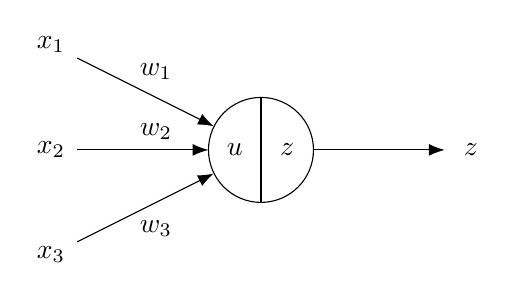
\begin{tikzpicture}[scale=1/3]
      \draw[-{Latex[length=2mm]}](-7,0)--(-2,0);
      \draw[-{Latex[length=2mm]}](-7,3.5)--(-1.8,0.9);
      \draw[-{Latex[length=2mm]}](-7,-3.5)--(-1.8,-0.9);
      \draw[-{Latex[length=2mm]}](2,0)--(7,0);
      \draw(0,2)--(0,-2);
      \draw (0,0) circle[radius=2];
      \draw (-1,0) node{$u$};
      \draw (1,0) node{$z$};
      \draw (8,0) node{$z$};
      \draw (-8,0) node{$x_2$};
      \draw (-8,4) node{$x_1$};
      \draw (-8,-4) node{$x_3$};
      \draw (-4,3) node{$w_1$};
      \draw (-4,0.7) node{$w_2$};
      \draw (-4,-3) node{$w_3$};
    \end{tikzpicture}
  \end{minipage}
  \begin{minipage}[b]{0.5\linewidth}
    \centering
    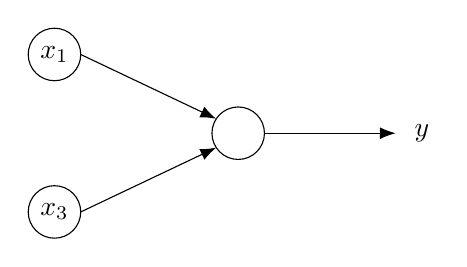
\begin{tikzpicture}[scale=1/3]
      \draw[-{Latex[length=2mm]}](-6,3)--(-0.84,0.55);
      \draw[-{Latex[length=2mm]}](-6,-3)--(-0.84,-0.55);
      \draw[-{Latex[length=2mm]}](1,0)--(6,0);
      \draw (0,0) circle[radius=1];
      \draw (-7,3) circle[radius=1];
      \draw (-7,-3) circle[radius=1];
      \draw (7,0) node{$y$};
      \draw (-7,3) node{$x_1$};
      \draw (-7,-3) node{$x_3$};
    \end{tikzpicture}
  \end{minipage}
  \caption{形式ニューロン(左)と簡単なニューロン回路(右)}
\end{figure}


\subsection{パーセプトロン}
形式ニューロンでどんな論理回路でも作ることがわかったが,どのようにニューロン回路を設計すれば,解きたい問題を計算してくれる効率的な回路が設計できるがはわからない.\par
そこでローゼンブラットは形式ニューロンのネットワークの重み$w$とバイアス$b$を解きたい問題に対してよく処理できるように訓練させるという「教師あり学習」のアイデアを付け加えた.\par
\begin{figure}
  \begin{center}
    \centering
    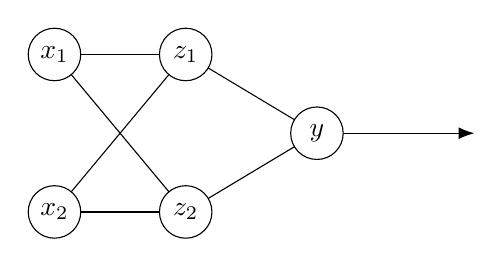
\begin{tikzpicture}[scale=1/3]
      \draw[-{Latex[length=2mm]}](-5,3)--(0,-3);
      \draw[-{Latex[length=2mm]}](-5,-3)--(-0,3);
      \draw[-{Latex[length=2mm]}](0,3)--(5,0);
      \draw[-{Latex[length=2mm]}](0,-3)--(5,0);
      \draw[-{Latex[length=2mm]}](-5,3)--(0,3);
      \draw[-{Latex[length=2mm]}](-5,-3)--(0,-3);
      \draw[-{Latex[length=2mm]}](6,0)--(11,0);
      \filldraw[fill=white] (0,3) circle[radius=1];
      \filldraw[fill=white] (0,-3) circle[radius=1];
      \filldraw[fill=white] (-5,3) circle[radius=1];
      \filldraw[fill=white] (-5,-3) circle[radius=1];
      \filldraw[fill=white] (5,0) circle[radius=1];
      \draw (0,3) node{$z_1$};
      \draw (0,-3) node{$z_2$};
      \draw (-5,3) node{$x_1$};
      \draw (-5,-3) node{$x_2$};
      \draw (5,0) node{$y$};
    \end{tikzpicture}
    \caption{2層からなるパーセプトロン}
    \label{2層パーセプトロン}
  \end{center}
\end{figure}
形式ニューロンを複数組み合わせることで作ったニューロン回路をパーセプトロンと呼ぶ.パーセプトロンは層構造をなしている.図\ref{2層パーセプトロン}は2層構造をもつパーセプトロンの例である.ただし,入力層は層数には数えない.丸の中には,その形式ニューロンの出力値が書かれている.\par
一般に,複数の形式ニューロンの集まりからなる層の出力は,隣接する次の層の形式ニューロンへ入力する.各層からの出力が,また次層へと入力する構造を繰り返す.ただし,はじめの層は入力層と呼ばれ,入力値のベクトル$\bm{x}^{\top}=(x_1, x_2, \cdots)$の各成分$x_i$を出力値としてもつ,入力用の形式ニューロンの集まりである.つまり入力層の形式ニューロンの数は,入力ベクトルの次元の数だけある.\par
一方,最後の出力は出力層と呼ばれる.推定したい最終結果$\bm{t}^{\top}=(y_1, y_2, \cdots)$の各成分$y_i$を出力値とする.それ以外の入出力間にある層は中間層や隠れ層と呼ばれる.各層のニューロン数については特に制限はない.図\ref{2層パーセプトロン}の例では2つのニューロンからなる入力層と中間層,そして1つのニューロンからなる出力層を持っている.重みパラメータを使って学習ができるパーセプトロンは大きな注目を集め,1960年代の第1次ニューラルネットのブームを巻き起こした.

\subsection{順伝播型ニューラルネットワーク}
ニューラルネットはユニット(unit)と呼ばれる素子からなる.図\ref{順伝播ニューラルネットワーク}(左)に示したユニットは,パーセプトロンにおける形式ニューロンに他ならない.ただし各ユニットは実数値の入出力をもつ.つまり各ユニットの出力値として,どんな実数を考えてもよいということである.もう1つの大きな違いは,活性化関数として微分可能は増化関数を採用するということである.例えばシグモイド関数がよく用いられていた.まず,ユニットにさまざまな入力$x_i$は入ってきているとする.各ユニットによって結合強度が異なるため,実際にはそれらの重み付き和
\begin{equation}
  u = \sum_{i} w_i x_i
\end{equation}
がユニットへの総入力となる.$u$は活性とも呼ばれる.この活性にバイアス$b$を加えたうえで,さらに活性化関数(activation function)$f$での変換を施したものが,このユニットからの出力$z$になる.
\begin{equation}
  z = f(u + b) = f\left( \sum_{i} w_i x_i + b \right)
\end{equation}
活性化関数は閾値$-b$を超えるとニューロンが信号を発することをモデル化する部分であるため,昔の研究では階段関数によく似た連続関数がよく用いられていた.その一例がシグモイド関数
\begin{equation}
  \sigma(u + b) = \frac{1}{1 + e^{-u-b}}
\end{equation}
である.図\ref{シグモイド関数}をみると,閾値付近で信号が立ち上がっていることがわかる.
\begin{figure}
  \begin{center}
    \centering
    \begin{tikzpicture}[scale=2,samples=300]
      \draw[->,>=stealth,semithick](-2,0)--(2,0)node[below]{$u$};%x軸
      \draw[->,>=stealth,semithick](0,-0.5)--(0,1.5)node[above]{$\sigma(u+b)$};%y軸
      \draw (-0.5,0.08)--(-0.5,-0.08)node[below]{-b};
      \draw (0.08,1)--(-0.08,1)node[left]{1};
      \draw (0,0)node[below left]{0};
      \draw[draw=magenta,thick,domain=-2:2] plot(\x,{1/(1+pow(e,-6*\x-3))});
    \end{tikzpicture}
    \caption{シグモイド関数}
    \label{シグモイド関数}
  \end{center}
\end{figure}



\begin{figure}[htbp]
  \centering
  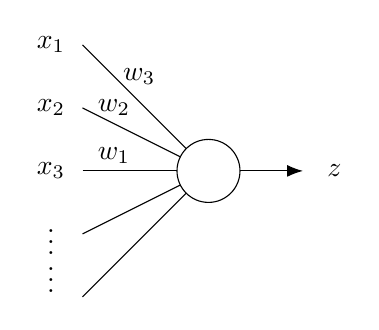
\begin{tikzpicture}[scale=1/2.5]
    \draw (-4,4)--(0,0);
    \draw (-4,2)--(0,0);
    \draw (-4,0)--(0,0);
    \draw (-4,-2)--(0,0);
    \draw (-4,-4)--(0,0);
    \draw[-{Latex[length=2mm]}] (1,0)--(3,0);
    \filldraw[fill=white] (0,0) circle[radius=1];
    \draw (-5,4) node{$x_1$};
    \draw (-5,2) node{$x_2$};
    \draw (-5,0) node{$x_3$};
    \draw (-3,0.5) node{$w_1$};
    \draw (-3,2) node{$w_2$};
    \draw (-2.2,3) node{$w_3$};
    \draw (4,0) node{$z$};
    \draw (-5,-2) node{$\vdots$};
    \draw (-5,-3.2) node{$\vdots$};
  \end{tikzpicture}
  \caption{ユニットの構造.$x_1,x_2,\dots$の入力を受け,$z$を出力する}
  \label{順伝播ニューラルネットワーク}
\end{figure}


\begin{figure}
  \begin{center}
    \centering
    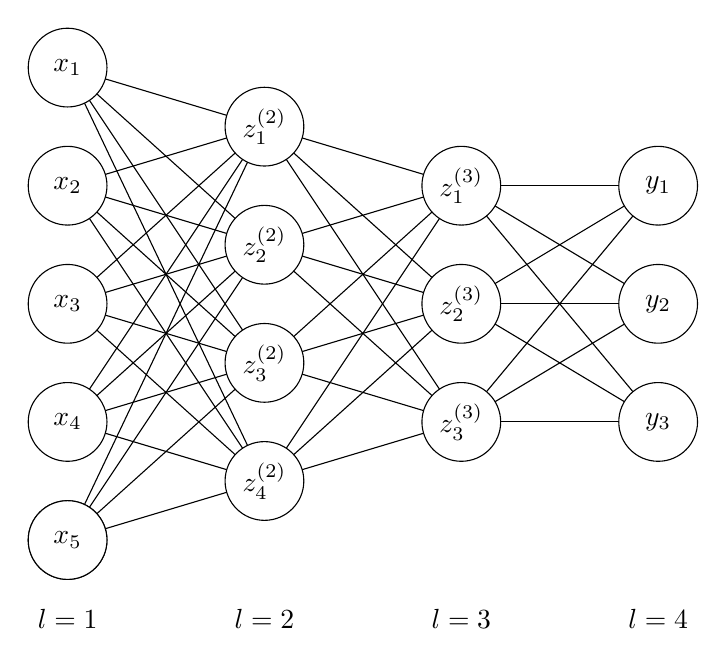
\begin{tikzpicture}[scale=1/2]
      \draw (0,0)--(5,1.5);
      \draw (0,0)--(5,4.5);
      \draw (0,0)--(5,7.5);
      \draw (0,0)--(5,10.5);
      \draw (0,3)--(5,1.5);
      \draw (0,3)--(5,4.5);
      \draw (0,3)--(5,7.5);
      \draw (0,3)--(5,10.5);
      \draw (0,6)--(5,1.5);
      \draw (0,6)--(5,4.5);
      \draw (0,6)--(5,7.5);
      \draw (0,6)--(5,10.5);
      \draw (0,9)--(5,1.5);
      \draw (0,9)--(5,4.5);
      \draw (0,9)--(5,7.5);
      \draw (0,9)--(5,10.5);
      \draw (0,12)--(5,1.5);
      \draw (0,12)--(5,4.5);
      \draw (0,12)--(5,7.5);
      \draw (0,12)--(5,10.5);
      \draw (5,1.5)--(10,3);
      \draw (5,1.5)--(10,6);
      \draw (5,1.5)--(10,9);
      \draw (5,4.5)--(10,3);
      \draw (5,4.5)--(10,6);
      \draw (5,4.5)--(10,9);
      \draw (5,7.5)--(10,3);
      \draw (5,7.5)--(10,6);
      \draw (5,7.5)--(10,9);
      \draw (5,10.5)--(10,3);
      \draw (5,10.5)--(10,6);
      \draw (5,10.5)--(10,9);
      \draw (10,3)--(15,3);
      \draw (10,3)--(15,6);
      \draw (10,3)--(15,9);
      \draw (10,6)--(15,3);
      \draw (10,6)--(15,6);
      \draw (10,6)--(15,9);
      \draw (10,9)--(15,3);
      \draw (10,9)--(15,6);
      \draw (10,9)--(15,9);
      \filldraw[fill=white] (0,0) circle[radius=1];
      \filldraw[fill=white] (0,3) circle[radius=1];
      \filldraw[fill=white] (0,6) circle[radius=1];
      \filldraw[fill=white] (0,9) circle[radius=1];
      \filldraw[fill=white] (0,12) circle[radius=1];
      \filldraw[fill=white] (5,1.5) circle[radius=1];
      \filldraw[fill=white] (5,4.5) circle[radius=1];
      \filldraw[fill=white] (5,7.5) circle[radius=1];
      \filldraw[fill=white] (5,10.5) circle[radius=1];
      \filldraw[fill=white] (10,3) circle[radius=1];
      \filldraw[fill=white] (10,6) circle[radius=1];
      \filldraw[fill=white] (10,9) circle[radius=1];
      \filldraw[fill=white] (15,3) circle[radius=1];
      \filldraw[fill=white] (15,6) circle[radius=1];
      \filldraw[fill=white] (15,9) circle[radius=1];
      \filldraw[fill=white] (0,0) circle[radius=1];
      \draw (0,0) node{$x_5$};
      \draw (0,3) node{$x_4$};
      \draw (0,6) node{$x_3$};
      \draw (0,9) node{$x_2$};
      \draw (0,12) node{$x_1$};
      \draw (5,1.5) node{$z_4^{(2)}$};
      \draw (5,4.5) node{$z_3^{(2)}$};
      \draw (5,7.5) node{$z_2^{(2)}$};
      \draw (5,10.5) node{$z_1^{(2)}$};
      \draw (10,3) node{$z_3^{(3)}$};
      \draw (10,6) node{$z_2^{(3)}$};
      \draw (10,9) node{$z_1^{(3)}$};
      \draw (15,3) node{$y_3$};
      \draw (15,6) node{$y_2$};
      \draw (15,9) node{$y_1$};
      \draw (0,-2) node{$l=1$};
      \draw (5,-2) node{$l=2$};
      \draw (10,-2) node{$l=3$};
      \draw (15,-2) node{$l=4$};
    \end{tikzpicture}
    \caption{入力層と3層からなる順伝播ニューラルネットワークの例.ユニットを表す丸の中に書かれた変数は,各ユニットの出力値を意味する.}
    \label{順伝播ニューラルネットワークの例}
  \end{center}
\end{figure}

順伝播ニューラルネット(feedforward neural network)はこのようなユニットを層状につなぎ合わせたアーキテクチャである.これを略してニューラルネットとも呼ぶ.図\ref{順伝播ニューラルネットワークの例}はその典型的な一例である.$l$が層数で,$l=1$が入力層,$l=4$が出力層,そして,$l=2,3$が中間層,または隠れ層である.信号の伝達は$l=1,2,3,4$の順に進み,そのため順伝播型と呼ばれる.\par
まず,入力層は5つのユニットからなっている.各ユニットはニューラルネット全体への入力ベクトル$\bm{x}^{\top}=(x_1, x_2, x_3, x_4, x_5)$の各成分を出力する.したがって入力ユニットは活性化関数をもたず,単に値$x_i$を出力するだけである.入力層はニューラルネットの層数には数えない.\par
入力層は入力ベクトル$\bm{x}$の次元数だけユニットをもつ.また,「第1層からの出力である」という意味を込めて次のようなラベル付けをする.
\begin{equation}
  \bm{z}^{(1)} = \bm{x}
\end{equation}
次に中間層について考える.第$l$層中の$j$番目のユニットを考える.このユニットは第$l-1$層の各ユニットからの入力$z_i^{(l-1)}$を入力として受けるため.活性は
\begin{equation}
  u_l^{(l)} = \sum_i w_{ji}^{(l)} z_i^{(l-1)}
\end{equation}
となる.ただし$w_{ji}^{(l)}$は,第$l-1$層のユニット$i$を第$l$層のユニット$j$の間の結合の重みである.\par
ユニットの出力は,活性$u_j^{(l)}$にユニット固有のバイアス$b_j^{(l)}$を加え,さらに活性化関数$f^{(l)}$を作用させたもの
\begin{equation}
  z_j^{(l)}
  = f^{(l)} \left( u_j^{(l)} + b_j^{(l)} \right)
  = f^{(l)} \left( \sum_i w_{ji}^{(l)} z_i^{(l-1)} + b_j^{(l)} \right)
\end{equation}
で与えられる.活性化関数は$f^{(l)}$はユニットごとに変えてもかまわないが,一般的には層ごとに共通の関数を用いる.\par
これらの式を行列表示しよう.まず$l$層の全ユニットの活性をまとめてベクトル$\bm{u}^{(l)}=\left( u_j^{(l)} \right)$で,出力をまとめて$\bm{z}^{(l)}=\left( z_j^{(l)} \right)$で表す.また,第$l-1$層のユニット$i$と第$l$層のユニット$j$の間の結合の重み$w_{ji}^{(l)}$を$(j,i)$成分とする重み行列
\begin{equation}
  \bm{W}^{(l)}
  =\begin{pmatrix}
    w_{11}^{(l)} & w_{11}^{(l)} & \cdots \\
    w_{21}^{(l)} & w_{22}^{(l)} &        \\
    \vdots       &              & \ddots \\
  \end{pmatrix}
\end{equation}
も導入する.さらにバイアスのまとめて縦ベクトル$\bm{b}^{(l)} = \left( b_j^{(l)} \right)$で表記することにすると,中間層が行う演算処理は
\begin{equation}
  \bm{u}^{(l)}
  = \bm{W}^{(l)} \bm{z}^{(l-1)}, \ \ \ \bm{z}^{(l)} = f^{(l)}\left( \bm{u}^{(l)} + \bm{b}^{(l)} \right)
\end{equation}
とまとめることができる.ただし,一般のベクトル$\bm{v}^{\top} = (v_1 v_2 v_3 \cdots)$に対する関数$f$の作用は,次のように各成分にそれぞれ作用するものとして定義することにする.\par
\begin{equation}
  f(\bm{v}) = f\begin{pmatrix}
    v_1 \\ v_2 \\ v_3 \\ \vdots
  \end{pmatrix} = \begin{pmatrix}
    (f(\bm{v}))_1 \\ (f(\bm{v}))_2 \\ (f(\bm{v}))_3 \\ \vdots
  \end{pmatrix} \equiv \begin{pmatrix}
    f(v_1) \\ f(v_2) \\ f(v_3) \\ \vdots
  \end{pmatrix}
\end{equation}
これまで重みとバイアスを区別して書いたが,バイアスも重みに含めてしまうことができる.それを理解するためにすべての中間層(と入力層)に,常に$1$という出力をするユニットを1つ加える.そしてそれを$i=0$というラベルで呼ぶことにする.
\begin{equation}
  z_0^{(l)} = 1
\end{equation}
第$l-1$層の$i=0$と第$l$層の$j \neq 0$の間に重み$w_{j0}^{l}$を導入する.すると,これはバイアスそのものになる.なぜなら$w_{j0}^l = b_j^l$とおくと,
\begin{equation}
  \sum_{i=0} w_{ji}^l z_i^{l-1}
  = \sum_{i=1} w_{ji}^l z_i^{l-1} + w_{j0}^l
  = \sum_{i=1} w_{ji}^l z_i^{l-1} + b_j^l
\end{equation}
となるからである.そのため,今後,必要のない場合は重みの中にバイアスも含めてしまい,バイアスをあらわに書かない次のような表記を用いることにする.\par
\begin{equation}
  \bm{u}^{(l)}
  = \bm{W}^{(l)} \bm{z}^{(l-1)}, \ \ \ \bm{z}^{(l)} = f^{(l)}\left( \bm{u}^{(l)} \right)
\end{equation}
最後に出力層について考える.$L-1$層からなる順伝播型ニューラルネットを考える.すると最後の第$L$層が出力層に相当する.出力層は,手前の第$L-1$層から$\bm{z}^{(L-1)}$を入力され,それを変換することでニューラルネットの最終出力$\bm{y}=\bm{z}^{(L-1)}$を出力する.出力層の役割は,回帰など機械学習で実行したいタスクを処理することである.つまり,$\bm{h}=\bm{z}^{(L-1)}$が入力$\bm{x}$の表現であり,この表現$\bm{h}$の回帰分析を通じて$\bm{x}$と$\bm{y}$の関係を推定するのが出力層の役割である.\par
\begin{equation}
  \hat{\bm{y}}
  = \bm{z}^{(L)}
  = f^{(L)}\left( \bm{u}^{(L)} \right), \ \ \
  \bm{u}^{(L)}
  = \bm{W}^{(L)} \bm{h}
\end{equation}
出力層においては,活性化関数の値域が目標変数の値域と一致するように$f^{(L)}$を選ぶ必要がある.\par
入力層から出力層に至る一連の情報処理の仕組みを説明した.結局のところ順伝播型ニューラルネットは,各総出の処理を順次入力ベクトル$\bm{x}$に施していくことで,$\bm{x}$から次の出力値を与える関数モデルということになる.
\begin{equation}
  \hat{\bm{y}}
  = f^{(L)}\left( \bm{W}^{(L)}f^{(L-1)} \left( \bm{W}^{(L-1)}f^{(L-2)} \left( \cdots \bm{W}^{(2)}f^{(1)(\bm{x})} \right) \right) \right)
\end{equation}

\section{ニューラルネットワークによる機械学習}
順伝播ニューラルネットは入力$\bm{x}$を受け取ると出力
\begin{equation}
  \bm{y}\left( \bm{x}; \bm{W}^{(2)},\dots ,\bm{W}^{(L)},\bm{b}^{(2)},\dots ,\bm{b}^{(L)} \right) \label{NN出力}
\end{equation}
を出す.出力地は重み$\bm{W}^{(l)}$やバイアス$\bm{b}^{(l)}$の値を変えることで変化する.これらのパラメータをまとめて$\bm{\theta}$と書くことにする.この出力を機械学習における識別関数とみなすと,データを用いてパラメータ$\bm{theta}$に関してフィッティングすることができる.この手順は通常の教師あり学習と同じであり,まず訓練データ$\mathcal{D}=\{ (\bm{x}_n, \bm{y}_n) \}_{n=1,\dots ,N}$を用意する.そのうえで訓練データ$\bm{x}_n$を入れた際のニューラルネットワークの出力値$\bm{y}(\bm{x}_n; \bm{\theta})$と,目標値$\bm{y}_n$のズレができるだけ小さくなるように,重みとバイアスを調整して学習する.ズレを測る誤差関数$E(\bm{\theta})$の選び方は,考えるタスクと出力層の構造に依存する.そして誤差関数の最小化
\begin{equation}
  \bm{\theta}^* = \underset{\bm{\theta}} {\operatorname{argmin}} \ E(\bm{\theta})
\end{equation}
が学習に対応する\par
式(\ref{NN出力})のように考えると,入力から一気に$\bm{y}$が得られているように見えるが,実際は層状の構造に従って信号が処理されていた.特に,第$L-1$層までの情報処理と,最後の出力層を切り分けて考えてみよう.なぜなら,第$L-1$層の部分までは,入力$\bm{x}$から層ごとに順次高次な表現を構成する役割を果たしているとみなせるからである.するともっとも最後の第$L-1$層からの出力は,入力$\bm{x}$に対する深層表現$\bm{h}$である.
\begin{equation}
  \bm{h}\left( \bm{x}; \bm{W}^{(2)},\dots ,\bm{W}^{(L-1)} \right)
  = \bm{z}^{(L-1)}\left( \bm{x}; \bm{W}^{(2)},\dots ,\bm{W}^{(L-1)} \right)
\end{equation}
すると出力層は,この表現を使って回帰のような通常の機械学習を行う役割を担っているとみなせる.\par
では次に,ニューラルネットワークにさせたいタスクごとに分けて,出力層の構造を見ていく.
\subsection*{回帰}
もし表現$\bm{h}$について線形回帰を行いたいのであれば,自明な活性化関数,つまり単なる恒等写像を用いた出力層を用意すればよい.
\begin{equation}
  \bm{y}
  = \bm{W}^{(L)} \bm{h}
\end{equation}
このようなユニットは線形ユニットと呼ばれる.ただし多くの場合は線形ではない一般的な回帰を行いたいため,何らかの非自明な活性化関数を考える.
\begin{equation}
  \bm{y}(\bm{x}; \bm{\theta})
  = f^{(L)}\left( \bm{W}^{(L)} \bm{h} \right)
\end{equation}
具体的にどのような$f^{(L)}$を選ぶかは,問題の性質に応じて我々が設定する必要がある.\par
出力をデータでフィッティングするには,$\bm{y}(\bm{x}; \bm{\theta})$を用いたモデルの予測値と実際のデータができるだけ近くなるように,平均二乗誤差を最小化する.
\begin{equation}
  E(\bm{\theta})
  = \frac{1}{2} \sum_{n=1}^N \left( \bm{y}(/bm{x}_n; \bm{\theta}) - \bm{y}_n \right)^2, \ \ \
  \bm{\theta}^* = \underset{\bm{\theta}} {\operatorname{argmin}} \ E(\bm{\theta})
\end{equation}
学習により得られた最適パラメータ$bm{\theta}^*$を代入したモデル$\bm{y}(\bm{x}; \bm{\theta}^*)$は,入力$\bm{x}$の値に応じて$\bm{y}$をよく予測できるようになるだろう.これが通常の回帰と異なるのは,回帰関数のパラメータだけでなく,表現を決める中間層の重みパラメータも同時に学習しているということである.これがニューラルネットワークによる表現学習である.

\subsection*{2値分類}
回帰と並んで代表的なタスクは,データを2つのクラスに分類する2値分類であった.ただし,2つのクラスに対応するラベル$y$の値は0か1の2値であるとする.ニューラルネットワークで2値分類を表現するには,出力層が表現$\bm{h} = \bm{z}^{(L-1)}$のロジスティック回帰を与えるようにデザインすればよい.\par
訓練データ$\mathcal{D} = \{ (\bm{x}_n, y_n) \}_{n=1,\dots ,N}$の標準値$y_n$は0か1だが,ロジスティック回帰では,この2値変数そのものではなく,$y$が1である確率$\hat{y} = P(y=1 | \bm{x})$を推定する.言い換えれば$y$の期待値を推定する.なぜなら,2値変数$\mathrm{y}$の従うベルヌーイ分布のもとで期待値は$E_{P(y | \bm{x})}[\mathrm{y} | \bm{x}] = \sum_{y=0,1} y P(y | \bm{x}) = P(y=1 | \bm{x})$となるからである.したがってロジスティック回帰を行うには,出力層のユニットが1つでその出力値が$P(y=1 | \bm{x})$を推定するようなニューラルネットワークを考えるのが自然である.つまり,出力層の構造は式(\ref{})に合わせて,次のようにすればよい.
\begin{equation}
  y(\bm{x}; \bm{\theta})
  = P(y=1 | \bm{x}; \bm{\theta})
  = \sigma\left( \sum_i w_i^{(L)} h_i \right)
\end{equation}
このようなユニットはシグモイドユニットと呼ばれる.シグモイドユニットの活性化関数はまさにロジスティック回帰におけるシグモイド関数であり,ユニットへの対数オッズである.\par
\begin{equation}
  f^{(L)} = \sigma, \ \ \
  u^{(L)}(\bm{x}; \bm{\theta}) = \ln{\frac{P(y=1 | \bm{x}; \bm{\theta})}{1 - P(y=1 | \bm{x}; \bm{\theta})}}
\end{equation}
このニューラルネットワークが訓練できれば,学習済みモデルに分析したいデータ$\bm{x}$を入力した際の出力値から,$\bm{x}$のどちらのクラスに属するかを判定できる.なぜならば,$P(y=1 | \bm{x})$が1/2を越えれば$y=1$のクラス,下回れば$y=0$のクラスに属するのが尤もらしいと判断できるからである.\par
ではこのようなニューラルネットワークはどのように学習させればよいか.出力層はロジスティック回帰の構造をもっているため,ロジスティック回帰同様,最尤法を用いればよいことがわかる.つまり,ニューラルネットワークが$P(y=1 | \bm{x};\bm{\theta})$を推定するベルヌーイ分布
\begin{equation}
  P(y | \bm{x}; \bm{\theta})
  = P(y = 1 | \bm{x}; \bm{\theta})^y (1 - P(y = 1 | \bm{x}; \bm{\theta}))^{(1-y)}
\end{equation}
を推定することと同じであるため,この分布の負の対数尤度を誤差関数にすればよい.したがって出力$y(\bm{x}_n; \bm{\theta}) = P(y=1 | \bm{x}_n; \bm{\theta})$に対し,
\begin{equation}
  E(\bm{\theta})
  = -\sum_{n=1}^N \left( y_n \ln{y(\bm{x}_n; \bm{\theta})}
  + (1 - y_n) \ln{1 - y(\bm{x}_n; \bm{\theta})} \right)
\end{equation}
が誤差関数であり,これを最小化するパラメータを見つけることが学習である.\par
このようにニューラルネットワークによって,ロジスティック回帰に向いた深層表現を表現学習できることになる.

\subsection*{多クラス分類}
最後に多クラス分類について考える.例えば手書き文字認識や画像認識は典型的な多クラス分類である.いまクラスが$K$個だけあるとする.$K$が3以上の場合は,表現$\bm{h}=\bm{z}^{(L-1)}$をソフトマックス回帰する出力層を作ればよい.\par
各クラスに対して目標変数が$y=1,2,\dots,K$という値をとるものとする.そして出力層には$K$個のユニットを用意し,それらの各ユニットは出力値として,入力$\bm{x}$が$y=k$番目のクラスに属する確率$P(y=k | \bm{x})$を推定するものとする.この出力層でソフトマックス回帰を表現するためには,出力層の$k$番目のユニットは次の出力値をもてばよい.
\begin{align}
  y_k(\bm{x}; \bm{\theta}) = P(y=k | \bm{x}; \bm{\theta})
  = \text{softmax}_k \left( u_1^{(L)},\dots ,u_K^{(L)} \right) \\
  \bm{u}^{(L)} = \bm{W}^{(L)} \bm{h}
\end{align}
ここで出力層の活性化関数はソフトマックス関数である.学習済みニューラルネットワークへ分析したいデータ$\bm{x}$を入力し,出力$y_k$が最大になる$k$を所属クラスと判定する.\par
ソフトマックス関数には,目標変数をベクトル表示するのが便利である.
\begin{equation}
  y \ \ \longleftrightarrow \ \
  \bm{t}(y)
  = (t(y)_j)
  = \begin{pmatrix}
    0 & \cdots & 0 & 1 & 0 & \cdots & 0
  \end{pmatrix}^{\top}
\end{equation}
右辺は$y=k$のとき,第$k$成分のみが1で他の成分は0のベクトルである.訓練データも,この$t$にかんして与えることにする.
\begin{equation}
  \mathcal{D}
  = \{ (\bm{x}_n, \bm{t}_n) \}_{n=1,\dots,N}
\end{equation}
このベクトル$\bm{t}_n$の第$k$成分を$t_{n,k}$と書くと,ニューラルネットワークのソフトマックス出力に対する交差エントロピーは
\begin{equation}
  E(\bm{\theta}) = -\sum_{n=1}^N \sum_{k=1}^K t_{n,k} \ln{y_k}(\bm{x}_n; \bm{\theta})
\end{equation}
であり,これが誤差関数に他ならない.



\subsection{活性化関数}

\section{畳み込みニューラルネットワーク}

\section{勾配降下法}
ニューラルネットワークの学習は損失関数の最小化によって行われる.つまり,ネットワークパラメータの空間上でスカラー関数$L(\bm{\theta})$の最小値を探すという最適化問題を解くことになる.
\begin{equation}
  \bm{\theta}^* = \underset{\bm{\theta}} {\operatorname{argmin}} \ L(\bm{\theta})
\end{equation}
損失関数は基本的に多くのパラメータを含む複雑な関数であるため,このような最適化問題を厳密に解くことはできない.そのため,計算機によって数値的に近似解を求めることになる.\par

\subsection{勾配降下法}
誤差関数$E(\bm{\theta})$の最小点を見つける手法のうち,最も直観的で単純なアイデアは図\ref{}のように,誤差関数のグラフの形状をした凹みにおいて.上のほうからボールを転がり落してボールの一番低いところにたどり着くまで待つ方法である.これがまさに勾配降下法の考え方である.\par

\begin{figure}
  \begin{center}
    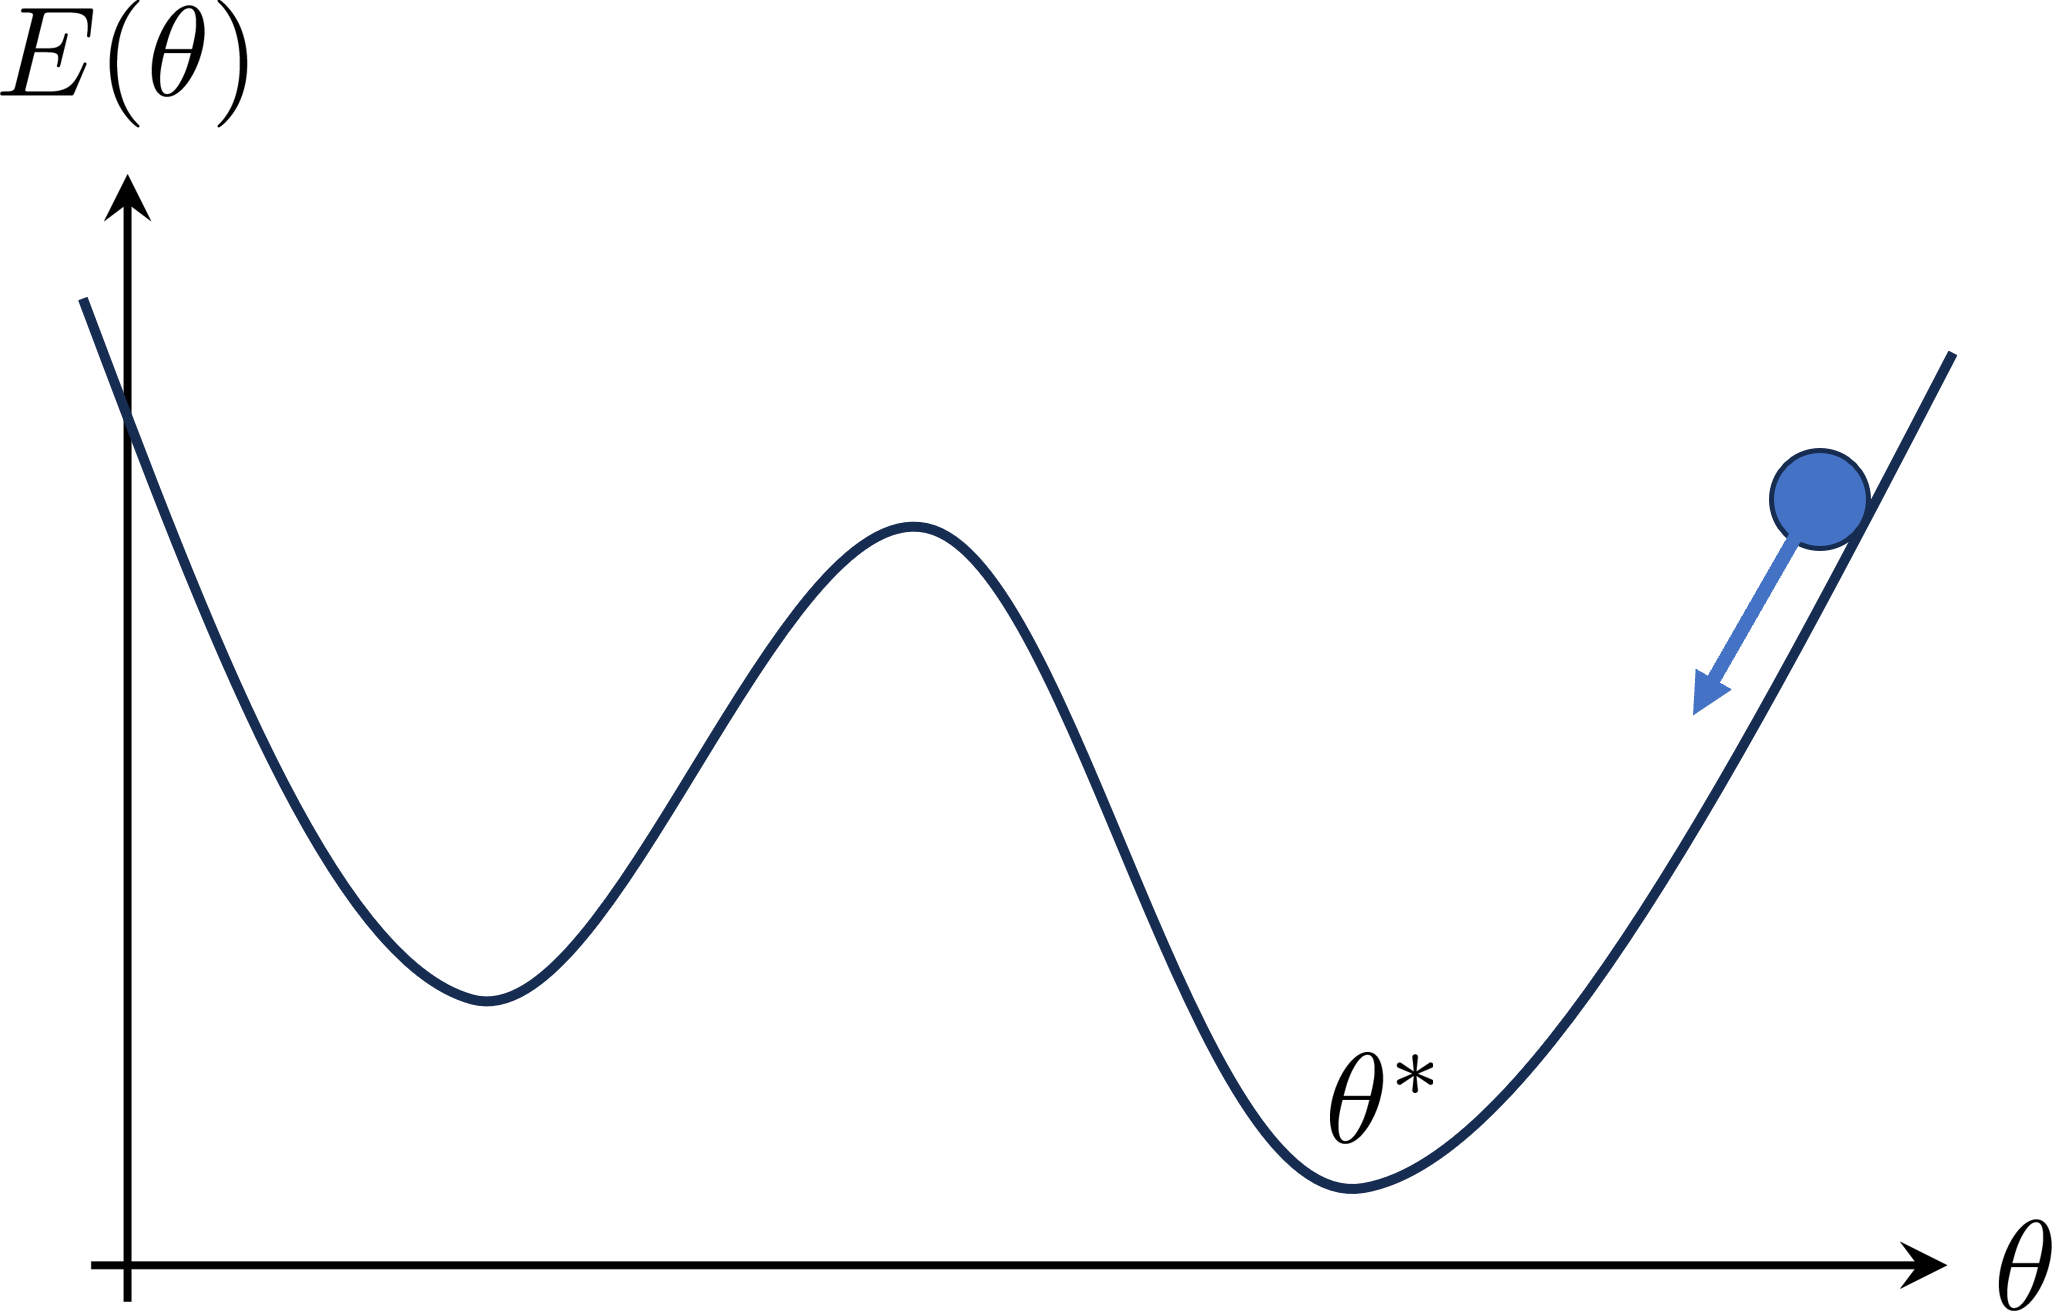
\includegraphics[height=5cm]{image/gradient_decent.png}
    \caption{勾配降下法による極小値の見つけ方}
  \end{center}
\end{figure}

ボールを転がり始めさせる位置に対応して,勾配降下法ではパラメータの初期値$\theta^{(0)}$を用意する.この初期値から始めて,坂道でボールを転がすような操作を,離散的な時間$t=0,1,2,\dots$を用いて定式化しよう.坂を転がすというのは,現在位置におけるグラフの勾配
\begin{equation}
  \nabla E(\bm{\theta})
  = \frac{\partial E(\bm{\theta})}{\partial \bm{\theta}}
  \equiv \left(  \frac{\partial E(\bm{\theta})}{\partial \theta_1}, \cdots,  \frac{\partial E(\bm{\theta})}{\partial \theta_D} \right)
\end{equation}
の逆方向に動かすことを意味する.ここで表記を簡単にするため,ニューラルネットワークの重みパラメータを下付き添え字$\theta_1,\theta_2,\dots,\theta_D$でラベル付けした.$D$はニューラルネットワークの全パラメータ数である.すると時刻$t$で位置$\bm{\theta^{(t)}}$にあったボールを勾配の逆方向に動かす際のルールは次のようになる.
\begin{equation}
  \bm{\theta^{(t+1)}} = \bm{\theta^{(t)}} + \Delta \bm{\theta^{(t)}} , \ \  \Delta \bm{\theta^{(t)}} = - \eta \nabla E\left( \bm{\theta}^{(t)} \right)
\end{equation}
右辺で次時刻の$\theta^{(t+1)}$を定義する操作を$t=0,1,2,\dots$と順次繰り返していくことで,どんどんと誤差関数のグラフの底のほうに降りていくことができる.$1$ステップでの移動距離$\Delta \bm{\theta^{(t)}}$の大きさを決めるハイパーパラメータ$\eta$は学習率(learning late)と呼ばれる.この操作が収束し,もはや動けなくなった点が勾配が消える極小値である.ここでいう収束とは,計算機の数値制度の範囲内でもはや$\theta^{(t)}$の変化が見られなくなる状況のことである.\par
学習率の取り方には一般論は存在せず,現状ではトライアルアンドエラーに基づかざるを得ない.しかし学習率をあまり大きくすると,$1$ステップの刻みが荒らすぎて誤差関数の形状をうまく捉えられずに,収束に問題を起こす.その一方であまり小さくしすぎると学習が一向に進まなくなる.したがって,程よい大きさの学習率を見つけることが,学習をうまく進めるために重要となる.\par

\subsection{局所的最小値の問題}
いままでは最小値と極小値の区別に注意を払わなかった.誤差関数が下に凸な関数である簡単な状況では任意の極小値は必ず最小値に一致するので区別する必要がない.しかしながらディープラーニングにおける誤差関数は一般的にとても複雑な非凸関数なので,本当の極小値である大域的極小値以外にも,膨大な数の局所的極小値をもつ.\par
さらにニューラルネットワークには高い対称性と極小値の重複がある.例えば,第$l$層の2つのユニット$j=1,2$に注目すると,この2つのユニットを入れ替えても最終層の出力は変わらない.なぜなら,$\theta_{1i}^{(l)},\theta_{k1}^{(l+1)}$と$\theta_{2i}^{(l)},\theta_{k2}^{(l+1)}$をすべて同時に入れ替えれば何もしていないことと同じになるからである.各層でこのような入れ替えは${}_{d_l} C_2$通りだけある.したがってニューラルネットワーク全体では$\prod_l {}_{d_l} C_2$通りだけの入れ替え対称性があることがわかる.つまり,局所的極小値が1つでも見つかれば,自動的に$\prod_l {}_{d_l} C_2$個の極小値が重複して存在することになる.このように,深層モデルでは極小値の数は膨大になる.\par
このような場合,勾配降下法で大域的極小値を探すのは,干草の中から針を探すようなものである.したがってディープラーニングでは極小値にはたどり着けても,真の極小値にはまずたどり着けない.通常の機械学習の文脈ではこれは深刻な問題であり,局所的最小値の問題や局所的最適解の問題と呼ばれる.\par
ところが不思議なことに,ディープラーニングでは真の最小値を見つけずとも,誤差関数のよい極小値さえ見つけられれば十分であると予想されている.これはディープラーニングを他の機械学習とは一線を画す画期的な手法にしていると同時に,ディープラーニングにおける大きな謎の1つである.この点に関しては現在でもさまざまな研究がなされている.\par

\subsection{確率的勾配降下法}
ディープラーニングが真の最小値を必要としないとはいっても,誤差関数の値があまりに大きい臨界点にはまり込んでしまっては全く使い物にならない.そこで臨界点にトラップされることをできるだけ回避するためにランダムな要素を取り入れて,はまり込んだ場所から弾き出す効果を生み出すことで勾配降下法を改良していく.\par
ランダムな要素を入れるためには,学習の仕組みを復習する必要がある.学習データ$\mathcal{D}=\{(\bm{x}_n,\bm{y}_n)\}_{n=1,2,\dots,N}$が与えられたとき,誤差関数は各学習サンプル要素$(\bm{x}_n,\bm{y}_n)$で計算した誤差の和として表現できた.
\begin{equation}
  E(\bm{\theta}) = \frac{1}{N}\sum_{n=1}^{N}E_n(\bm{\bm{\theta}}) \label{勾配降下法}
\end{equation}
例えば平均二乗誤差を用いるならば
\begin{equation}
  E_n(\bm{\bm{\theta}}) = \frac{1}{2}\left( \bm{y}(\bm{x}_n ; \bm{\theta}) - \bm{y}_n \right)^2
\end{equation}
であり,$K$クラス分類ならば交差エントロピー
\begin{equation}
  E_n(\bm{\bm{\theta}}) = - \sum_{k=1}^{K} t_{nk}\log{y_k(\bm{x}_n ; \bm{\theta})}
\end{equation}
を用いた.先ほどの勾配降下法では式(\ref{勾配降下法})のように毎回の更新ですべての訓練サンプルを用いていた.このような方法はバッチ学習と呼ばれる.\par
しかし勾配によるパラメータ更新は何回も繰り返すことになるので,1回の更新で毎回すべてのサンプルを用いる必要がない.各時間ステップで,一部の訓練サンプルだけを用いる方法をミニバッチ学習という.ミニバッチ学習ではまず,各時間$t$で用いる訓練サンプルの部分集合$\mathcal{B}^{(t)}$を用意する.この$\mathcal{B}^{(t)}$のことをミニバッチと呼び,通常は学習前にランダムに作成しておく,そして時刻$t$における更新ではミニバッチ上で平均した誤差関数
\begin{equation}
  E^{(t)}(\bm{\theta}) = \frac{1}{\mathcal{B}^{(t)}} \sum_{n\in \mathcal{B}^{(t)}} E_n(\bm{\theta})
\end{equation}
を用いる.ここで$n\in \mathcal{B}^{(t)}$はミニバッチに含まれる訓練サンプルのラベルを表し,$|\mathcal{B}^{(t)}|$はミニバッチの中のサンプル要素の総数である.これを用いてバッチ学習同様,パラメータを更新する.
\begin{equation}
  \bm{\theta^{(t+1)}} = \bm{\theta^{(t)}} + \Delta \bm{\theta^{(t)}} , \ \  \Delta \bm{\theta^{(t)}} = - \varepsilon \nabla E^{(t)}\left( \bm{\theta}^{(t)} \right)
\end{equation}
特に各時刻のミニバッチに1つの訓練サンプルしか含まない$|\mathcal{B}^{(t)}|=1$という場合をオンライン学習や確率的勾配降下法と呼ぶ.\par
ミニバッチ学習ではランダムにミニバッチを選んだことにより,時刻ごとに誤差関数$E^{(t)}(\bm{\theta})$の形もランダムに変化する.したがって,ずっと同じ関数$E(\bm{\theta})$を使い続けるバッチ学習とは違い,望ましくない臨界点にはまり込む可能性がかなり小さくなる.これがミニバッチ学習が重宝される大きな理由である.\par
さらにサンプルを効率的に使う観点からもミニバッチは好まれる.訓練データのサイズが大きくなると,似たようなサンプルが含まれる可能性が高くなる.そこで訓練データ集合全体ではなく,ミニバッチを使用することで,1回の更新ステップにおいて似たデータを重複して使用する無駄が省けるようになる.\par
またミニバッチでの勾配降下法では,各勾配$\nabla E_n(\bm{\theta})$の計算が独立で容易に並列化できる.したがって,コアのたくさんあるGPGPUなどの並列計算環境がある場合には,ある程度のサイズのミニバッチを利用するほうが理にかなっている.

\subsection{ミニバッチの作り方}
(ミニ)バッチ学習では,学習時間をエポック(epoch)という単位ごとに分けて考える.1エポックという単位は,訓練データ全体を1周すべて使い切る時間単位を意味する.\par
まずはじめのエポックでは,データを適当なサイズのミニバッチにランダムに分割する.そして,これらのミニバッチを用いて勾配を更新していく.すべてのミニバッチを使い切ったら,このエポックは終了になる.しかし通常は,1エポックでは不十分で,次のエポックに進み,改めてランダムにミニバッチを作り,同じプロセスを繰り返していく,そして,誤差関数が十分小さくなるまでエポックを繰り返したら,学習終了になる.\par
また,バッチ学習では毎回データを使い切るため,エポックと更新時間は一致する.

\section{改良された勾配降下法}
\subsection{勾配降下法の課題}
前節で勾配法には,局所最適解の問題があることをみたが,それ以外にも多くの課題がある.\par
図\ref{勾配法の課題}(a)のように誤差関数が深い谷を作っている状況を考える.このような谷に対して勾配降下法で勾配の方向にパラメータを更新するだけでは谷に沿って激しく振動するばかりで,いつまでたってもパラメータが収束しない.\par
一方,図\ref{勾配法の課題}(b)のように,平らな領域があった場合を考える.このような場所はプラトーと呼ばれる.一度プラトーに入り込んでしまうと勾配が消えるため,パラメータの更新も止まってしまう.ミニバッチアドでランダムな要素を入れたとしても,深層学習の誤差関数に現れるプラトーは学習の進みを遅くする原因になってしまう.\par
さらに,図\ref{勾配法の課題}(c)のような急に切り立った絶壁の存在も危険である.それまで緩やかな坂を下ってきたとしても,絶壁に当たった瞬間に極めて大きな勾配によって吹き飛ばされてしまう.
\begin{figure}[htbp]
  \begin{minipage}[b]{0.3\linewidth}
    \centering
    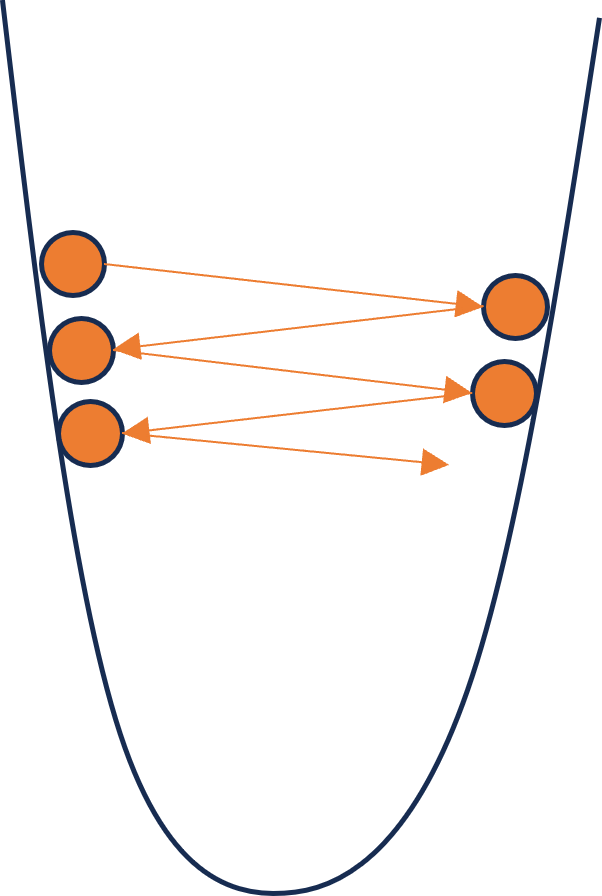
\includegraphics[keepaspectratio, scale=0.5]{image/勾配法課題(a)}
    \subcaption{}
  \end{minipage}
  \begin{minipage}[b]{0.3\linewidth}
    \centering
    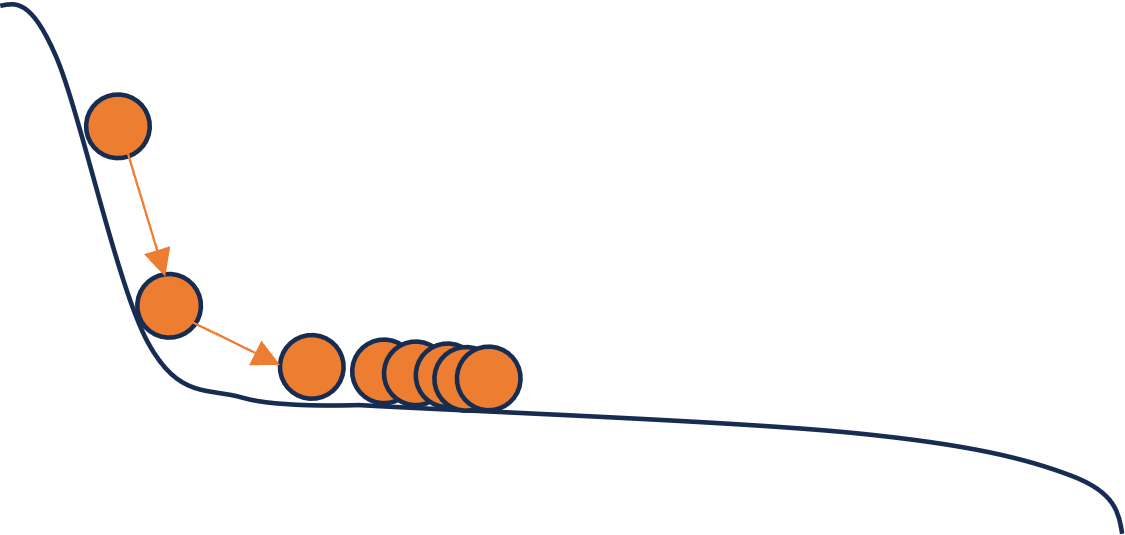
\includegraphics[keepaspectratio, scale=0.5]{image/勾配法課題(b)}
    \subcaption{}
  \end{minipage}
  \begin{minipage}[b]{0.3\linewidth}
    \centering
    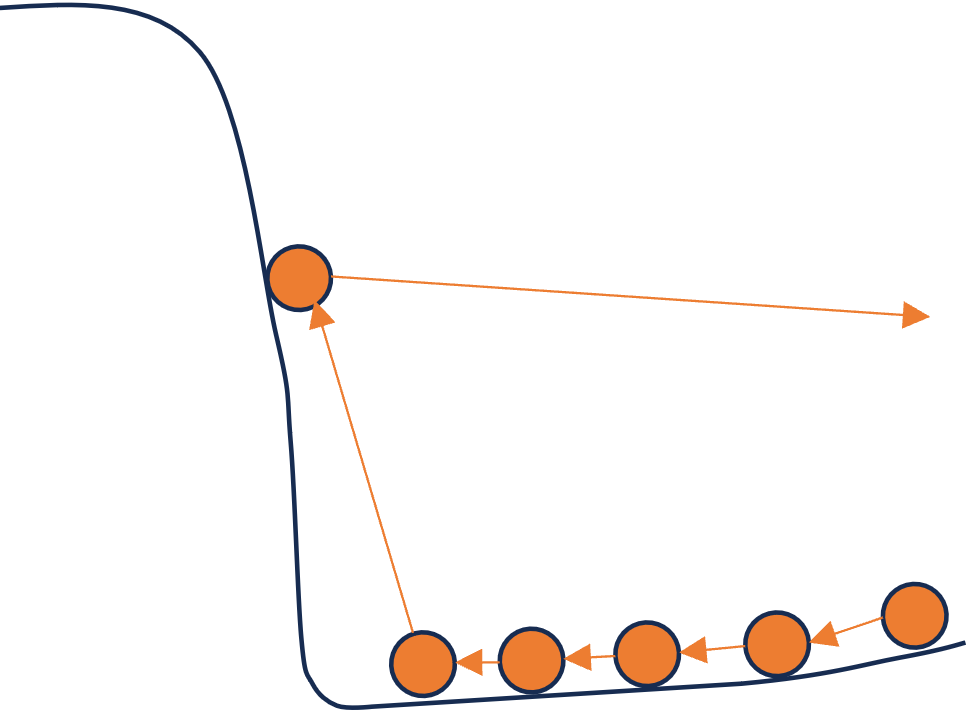
\includegraphics[keepaspectratio, scale=0.5]{image/勾配法課題(c)}
    \subcaption{}
  \end{minipage}
  \caption{(a)谷で振動.(b)プラトーで停止.(c)絶壁で反射}
  \label{勾配法の課題}
\end{figure}


\subsection{モーメンタム法}
振動による問題を改善する手法としてモーメンタム(momentum)というものがある.モーメンタムは「慣性」とも訳され.前時刻での勾配の影響を引きずらせることで振動を防ぐことができる.\par
振動の原因は,深い谷の底周りで急激な勾配が正負交互に発生するためであった.そこで,1個前のステップでの勾配の影響を,現在の勾配に加えることを考える.前回のパラメータ更新量$\Delta \bm{\theta}^{(t-1)}$が負の値で,現在の勾配$\nabla E(\bm{\theta}^{(t)})$が正の大きな値であるとする.すると前回の更新量を現在の勾配に少し加えることで,図\ref{モーメンタム法による勾配抑制図}のように今回の更新量$\Delta \bm{\theta}^{(t)}$を比較的小さな値に抑えることができる.つまり,手法で勾配が大きく正負に振れること防ぐことができる.
\begin{align}
  \bm{\theta}^{(t+1)}
   & = \bm{\theta}^{(t)} + \Delta \bm{\theta}^{(t)}                              \\
  \Delta \bm{\theta}^{(t)}
   & = \mu \Delta \bm{\theta}^{(t-1)} - (1-\mu) \eta \nabla E(\bm{\theta}^{(t)})
\end{align}
\begin{figure}
  \begin{center}
    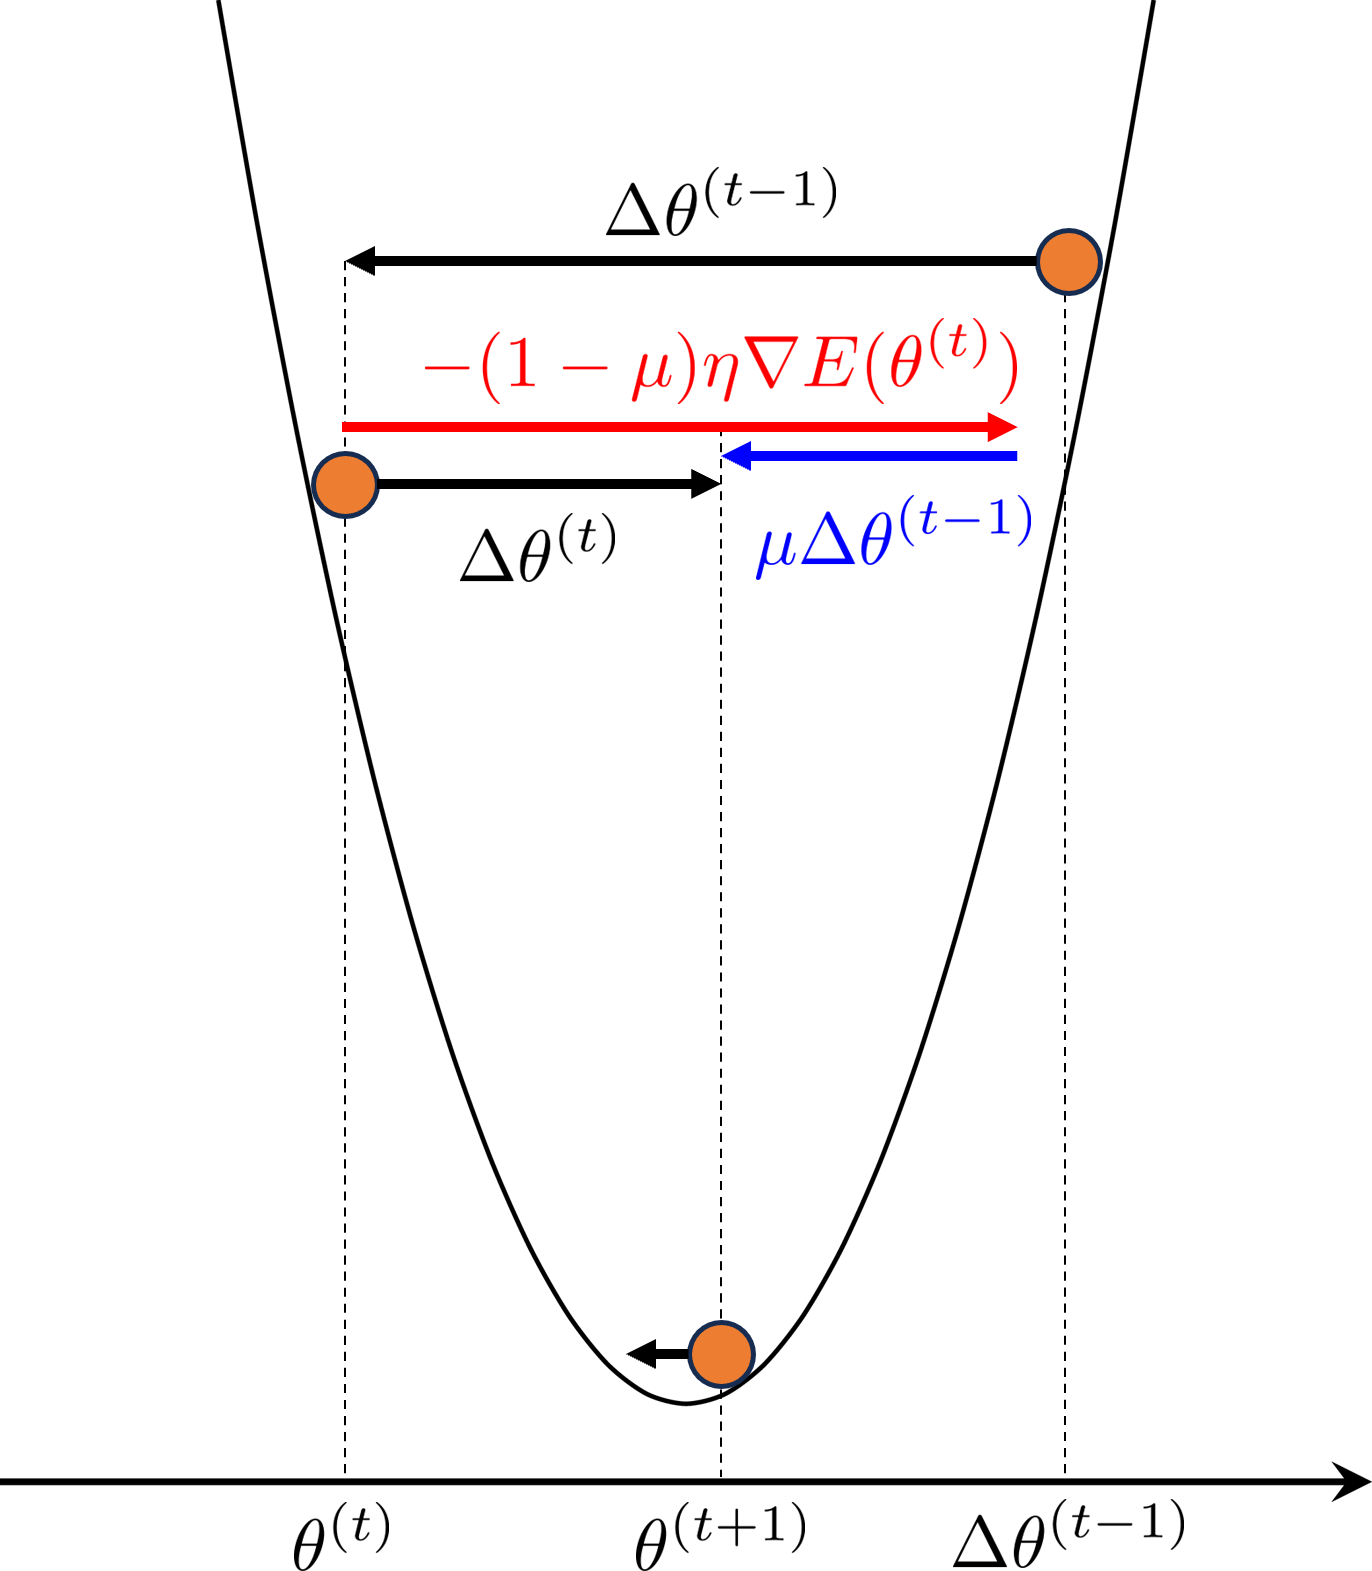
\includegraphics[height=8cm]{image/モーメンタム法.png}
    \caption{モーメンタム法による谷での振動の抑制}
    \label{モーメンタム法による勾配抑制図}
  \end{center}
\end{figure}
初期値は$\Delta \bm{\theta}^{(0)} = 0$にとる.また,$\mu$は比較的$1$に近い$0.5 \sim 0.99$程度の値をとる.\par
モーメンタム法は振動を防ぐ効果だけではなく,普通の斜面において勾配法でのパラメータ更新の加速も可能にする.これを見るために誤差関数の傾き$\nabla E(\bm{\theta}^{(t)})$が一定の領域を考える.この場合,式(\ref{})の終端速度は$\Delta \bm{\theta}^{(t)} = \Delta \bm{\theta}^{(t+1)} = \Delta \bm{\theta}$として更新式を解くことで,
\begin{equation}
  \Delta \bm{\theta} = -\eta \nabla E(\bm{\theta})
\end{equation}
となる.つまり傾きの一定の斜面では,もともとの式(\ref{})においては$(1-\mu)\eta$であった学習率が$\eta$にまで増える加速効果を与える.また,$\mu=0$にとるとモーメンタムの効果は消え,通常の勾配法に帰着する.

\subsection{AdaGrad}
モーメンタム法では勾配法の振動を防いだり,パラメータ更新を加速させたりする効果があった.ここでは,異なる側面に注目した改善策を説明する.\par
勾配降下法にはこれまで1つの学習率$\eta$しかなかった.しかし実際には,パラメータ空間の座標方向によって誤差関数の勾配に大きな違いが現れることが想定できる.例えば,$w_1$方向には急激な勾配を持つ一方,$w_2$方向には緩やかな傾きしか持たない誤差関数があったとする.すると$w_1$方向には大きな勾配に従い大きくパラメータ値が更新される一方,$w_2$方向には一向にパラメータ更新が進まない.これは勾配法をコントロールする学習率が1つしかないからである.\par
もし各パラメータ方向に応じて複数の学習率が導入できれば,どの方向にも均等な速度で学習を進めることができ,勾配降下法の収束性が良くなるはずである.ただし,むやみにやたらに学習率を増やしてしまっては,それらを我々がトライアンドエラーによって決めなくてはいけなくなり都合がよくない.そこでここでは,パラメータをあまり増やさずに,各方向に適切な有効学習率を持たせる手法を説明する.\par
このような手法のうち,早くから用いられていたものがAdaGrad(adaptive subgradient descent)である.
\begin{equation}
  \Delta \bm{\theta}_i^{(t)}
  = -\frac{\eta}{\sqrt{\sum_{s=1}^{t}\left(\nabla E(\bm{\theta}^{(s)})_i\right)^2}} \nabla E(\bm{\theta}^{(t)})
\end{equation}
左辺は$\Delta \bm{\theta}^{(t)}$の第$i$成分であり,$\nabla E(\bm{\theta}^{(t)})_i$は勾配の第$i$成分である.AdaGradでは,過去の勾配成分の二乗和の平方根で学習率を割っている.それにより,すでに大きな勾配値をとってきた方向に対しては勾配を小さく減少させ,いままで勾配の小さかった方向への学習率を増大させる効果がある.これにより,学習が一向に進まない方向が生じてしまうことを防ぐことができる\par
AdaGradの欠点をしては,学習の初期に勾配が大きいとすぐさま更新量$\Delta \bm{\theta}_i^{(t)}$が小さくなってしまうことである.そのままだと学習がストップするので,適切な程度にまで$\eta$を大きく選んであげる必要がある.そのためにAdaGradは学習率の選び方に敏感で使いにくい方法である.また,はじめから勾配が大きすぎるとすぐさま更新が進まなくなるため,重みの初期値にも敏感である.

\subsection{RMSprop}
RMSpropはヒントンにより講義の中で紹介された手法である.論文として出版していないにも関わらず,世界中で広く用いられている手法として有名である.\par
AdaGradの問題は,ひとたび更新が$0$になってしまったら二度と有限の値に戻らないことであった.これは過去のすべての勾配の情報を収集してしまっていたためである.そこで十分過去の勾配の情報を指数的な減衰因子によって消滅させるように,二乗和ではなく指数的な移動平均$v_{i,t}$から決まるroot mean square(RMS)を用いることにする.
\begin{align}
   & v_{i,t}
  = \rho v_{i,t-1} + (1-\rho) (\nabla E(\bm{\theta^{(t)}})_i)^2 \\
   & \Delta \bm{\theta}_i^{(t)}
  = - \frac{\eta}{\sqrt{v_{i,t}+\epsilon}} \nabla E(\bm{\theta^{(t)}})_i
\end{align}
初期値は$v_{i,0}=0$とする.また,$\epsilon$は分母が$0$とならないように導入した.よく$\epsilon = 10^{-6}$の値が用いられる.また簡単のために
\begin{equation}
  \mathrm{RMS}[\nabla E_i]_t = \sqrt{v_{i,t} + \epsilon}
\end{equation}
という記法を今後用いる.\par
RMSpropでは最近の勾配の履歴のみが影響するため,更新量が完全に消えてしまうことはない.また,深層学習では,うまく鞍点を抜け出した阿多は更新を加速したいため,モーメンタム法などと組み合わせて用いられる.RMSpropの有効性は広く実証されている.

\subsection{AdaDelta}
RMSpropはAdaGradを改善したとても良い方法である.しかしながら,全体の学習率$\eta$の値に敏感であるという事実にはあまり改善が見られない.その理由の1つは,次元性のミスマッチである.物理における次元解析を思い出そう.いま誤差関数$E$は無次元であるとする.つまりパラメータ$\bm{\theta}$を測るスケールを何倍しても不変な関数とする.その一方$\Delta \bm{\theta}$は長さの次元を持っており,$E$の微分は長さの逆数の次元を持つ.
\begin{equation}
  [\Delta \bm{\theta}] = \mathrm{L}, \ \ \ [\nabla E(\bm{\theta})] = \mathrm{L}^{-1}
\end{equation}
\subsection{Adam}
しかし,勾配法では,この次元性を合わない両者を学習率で比例させてしまっている.このミスマッチが学習率に押し付けられてしまうために,適切な学習率のスケールが問題に応じてさまざまに変化してしまうのである.\par
ロバストな学習率を実現させるためには,このミスマッチを解消しなくてはいけない.そこで

\section{誤差逆伝播法}


% \section{ボルツマンマシンの基礎}

\chapter{機械学習によるイジング模型の相転移検出}
\section{配位データの生成方法}
\section{相の分類器による相転移検出}
\section{温度測定器による相転移検出}
\section{相転移検出がなぜ可能なのか?}

% \chapter{機械学習と繰り込み群}
% \section{繰り込み群と特徴抽出}


\chapter*{まとめ}
研究のまとめを書く.

%=====================================================================================
\chapter*{謝辞} %章を付けずにタイトル表示
\addcontentsline{toc}{chapter}{謝辞} %章立てせずに目次に追加するおまじない
謝辞を書く.

%=====================================================================================

% \addcontentsline{toc}{chapter}{参考文献} %章立てせずに目次に追加するおまじない
\renewcommand{\bibname}{参考文献} %これがないと,タイトルが「関連図書」になってしまう
\bibliography{reference} %bibtexファイルの読み込み
\bibliographystyle{junsrt} %本文に\cite{}を入れることで,参考文献表示

% 付録
\appendix
\renewcommand{\thechapter}{\Alph{chapter}}
\renewcommand{\thesection}{\Alph{chapter}.\arabic{section}}
\setcounter{section}{0}
\renewcommand{\theequation}{\Alph{chapter}.\arabic{equation}}
\setcounter{equation}{0}

\chapter{aaa}
aaa
\section{bbb}
bbb


\end{document}